\documentclass[subeqn]{article}

\title{The Twin Instrument\footnote{We are grateful to Paul Devereux, James 
Fenske, Judith Hall, Cheti Nicoletti, Carol Propper, Atheen Venkataramani, 
Marcos Vera-Hernandez, Frank Windmeijer, Emilia Del Bono, Climent 
Quintana-Domeque, Pedro R\'odenas, Libertad Gonz\'alez, Hanna M\"uhlrad, 
Anna Aevarsdottir, Martin Foureaux Koppensteiner, Ryan Palmer and Pietro 
Biroli along with various seminar audiences and discussants for helpful 
comments and/or sharing data. All remaining errors are our own.}}
\author{Sonia Bhalotra\thanks{Department of Economics and ISER, The University of
    Essex. Contact: \href{mailto:srbhal@essex.ac.uk}{srbhal@essex.ac.uk}} 
\and Damian Clarke\thanks{Deparment of Economics, Universidad de Santiago de Chile.
Contact: \href{mailto:damian.clarke@usach.cl}
{damian.clarke@economics.ox.ac.uk}}}
\date{August 2015}

%at CMPO Bristol, ESPE, NEUDC, CSAE, The University of Essex, The University of 
%Oxford, the Barcelona GSE summer forum, PacDev, and the RES conference

%*******************************************************************************
\usepackage{amsmath}
\usepackage{amssymb}
\usepackage{appendix}
\usepackage{blindtext}
\usepackage{bm}
\usepackage{booktabs}
\usepackage{breqn}
\usepackage{caption}
\usepackage[usenames, dvipsnames]{color} \pagecolor{white}
\usepackage{dcolumn}
\usepackage{epsfig}
\usepackage{epstopdf}
\usepackage[capposition=top]{floatrow}
\usepackage{hyperref}
\usepackage{lastpage}
\usepackage{longtable}
\usepackage{lscape}
\usepackage{multirow}
\usepackage{natbib} \bibliographystyle{abbrvnat}\bibpunct{(}{)}{;}{a}{,}{,}
\usepackage{pdfpages}
\usepackage{rotating}
\usepackage{setspace}
\usepackage{subcaption}
\usepackage{subfloat}
\usepackage{url}
\usepackage{wrapfig}
\usepackage{xr}
\externaldocument{onlineAppendix_Twins}

%*******************************************************************************
\setlength\topmargin{-0.375in}
\setlength\textheight{8.8in}
\setlength\textwidth{5.8in}
\setlength\oddsidemargin{0.4in}
\setlength\evensidemargin{-0.5in}
\setlength\parindent{0.25in}
\setlength\parskip{0.25in}

\hypersetup{                                                                                                    
    colorlinks=true,   
    linkcolor=BlueViolet,
    citecolor=BlueViolet,
    filecolor=BlueViolet,
    urlcolor=BlueViolet
}


\newcommand{\twinfolder}{"/home/damian/investigacion/Activa/Twins"}
\DeclareMathOperator{\plim}{plim}

%*******************************************************************************
\begin{document}
\begin{spacing}{1.4}

\maketitle
\vspace{-1cm}
%\begin{center}{\Large\textsc{Preliminary Draft}}\end{center}
\begin{abstract}
 The incidence of twins has been used to identify the impact of changes in 
 fertility on measures of investment in children born prior to the twins, and
 the emerging consensus in this literature is that there is no evidence of a
 quantity-quality (Q--Q) trade-off. We argue that the standard approach is 
 flawed. Even if twin conception is random, bringing twins to term is a function 
 of maternal health which is difficult to fully observe and which tends to be
 correlated with child quality, rendering the instrument invalid. The neglect
 of this fact in the existing literature will tend to lead to under-estimation 
 of the Q--Q trade-off and so could contribute to explaining the negative results
 in the literature. Our contention that women who produce twin births are
 positively selected is demonstrated using data from richer and poorer countries.
 Using large samples of microdata from developing countries and from the USA 
 which include indicators of maternal health characteristics and behaviours, we
 show that a significant trade-off emerges upon correcting for these biases. We
 show that this result is likely to be only a \emph{lower} bound of the true
 Q--Q trade-off and discuss how to estimate the size of these bounds. These
 results have important implications for twin studies in all contexts examined
 here.
\\
\end{abstract}
\hspace{4mm}\textbf{\small JEL codes}: J12,J13,C13,D13,I12. \\

\newpage
%*******************************************************************************
\section{Introduction}                             \label{TWINscn:intro}
Since the pioneering work of \citet{RosenzweigWolpin1980}, economists have 
attempted to leverage the occurrence of twin births to estimate the effect of 
family size on child outcomes. If twin births occur at random, their occurrence 
constitutes a fertility shock that is uncorrelated with family characteristics, 
including parental preferences, and other unobservables which may be related to 
child quality. This provides the exogenous variation (in quantity) required to 
estimate the quantity-quality model of \citet{Becker1960,BeckerLewis1973,
BeckerTomes1976}.  The essential idea of these studies is that the shadow price 
of child quality is increasing in child quality and \emph{vice versa}. Thus, by 
comparing those families who unexpectedly produced additional children with 
those who always produced one child per birth, it is argued that the effect of 
an additional sibling on a child's human capital attainment can be uniquely
identified.

However, the consistent estimation of this effect is based upon the untestable 
assumption that twinning is exogenous. This requires not only that twin 
conceptions are randomly assigned to families, but also that taking a twin
conception to term does not depend upon a woman's behaviours during pregnancy 
or on her endowments prior to pregnancy. This is at odds with the evidence.

We show that endowments and behaviours affect the chances of twins being born. 
In data from a large sample of developing countries, we show that taller women 
and women with a higher body-mass index are significantly more likely to give 
birth to twins.\footnote{Height is an index of the stock of health of a woman 
and is a function of investments over her growth period and, especially, the 
early years of her life (see references in \citet{BhalotraRawlings2013}).} 
Maternal health is likely to be an especially significant determinant of birth 
outcomes in poorer countries where many women are chronically under-nourished 
(an indicator of which is their final stature), exhibit anemia and low-BMI, and 
are prone to infections. In these conditions only relatively healthy women will 
have the resources to support a successful twin pregnancy. However, our critique 
applies to richer countries too. Using administrative data from the Scotland,
the USA, Sweden and Spain, and survey data from the UK and Chile, we find that 
women who are taller and less likely to engage in risky behaviours such as 
smoking, drug taking or alcohol consumption during pregnancy are significantly 
more likely to have a (live) twin birth \citep{BhalotraClarke2016}.\footnote{%
  Simiarly, it is well known 
that fertility treatments increase the likelihood of twinning. While we do not 
discuss this extensively here, we note that this is likely to be less of an 
identification challenge given that IVF treatment is an entirely observable 
behaviour, unlike maternal health and pregnancy behaviours, which are 
multidimensional and largely unobservable.}

Overall, our argument is that women who give birth to twins are positively 
selected and that the common tendency to ignore this will result in under-%
estimation of the Q--Q trade-off. We focus upon maternal health because no 
previous work has highlighted it as a determinant of twinning, and because it is 
inherently impossible to fully control for. Even if we had data that included 
all of the indicators of health we mention above, we may not observe whether 
women skip breakfast \citep{MazumderSeeskin2014}, whether they are stressed 
(\citet{Blacketal2014} and references therein), whether they seek and adhere to 
antenatal care and so on. Our contention adds a novel twist to a recent 
literature which suggests that mothers' health and fetal environment matter and 
may alter the birth weight of children, the sex ratio at birth and a range of 
future human capital outcomes \citep{Almondetal2011,BhalotraRawlings2013,
Barker1995}. Like birth weight and the probability of a boy relative to a girl 
birth, the probability of a twin birth is increasing in the health of the 
mother/the fetal environment.

The emerging consensus in the literature using twin births to test the Q--Q 
model is that there is in fact no significant or substantial trade-off between 
fertility and investments in children. In this paper we suggest that this result 
may, in principle, follow from the bias created by twin-mothers being positively 
selected. We re-examine the validity of these results, accounting for the 
innovation discussed previously.  If twin births are not truly exogenous, but 
instead depend upon maternal health stocks and behaviours, there is an 
identification challenge.  Specifically, if healthier mothers are both more 
likely to give birth to twins, and more likely to invest in child human capital 
in later life, existing estimates may significantly underestimate the size of 
the Q--Q trade-off.  When ignoring these considerations we find that the effect 
of an additional birth on human capital attainment (education) is minor, or even 
weakly positive. However, when taking into account this innovation we find that 
a significant trade-off does exist, and that an additional birth reduces 
standardised schooling behaviour by at least 4\% of a standard deviation.

\textcolor{red}{The magnitude of the effect of one additional birth is small 
but the total effect can be large in the context of high fertility.}


The estimated effect of $\sim 4\%$ of an s.d.\ is at most the lower bound for 
the true size of the Q--Q trade-off. Given that we suggest that maternal health 
predicts twinning, and given that maternal health is multidimensional in nature 
and difficult to observe fully, we will only ever be able to include a partial 
set of controls to account for the inconsistency in IV estimates. As such, we 
examine a number of methods to estimate plausible bounds on the Q--Q trade-off. 
First, we argue that the true estimate is bounded by the OLS and IV estimtes. 
We also follow \citet{Conleyetal2012} in conceptualizing twins as a plausibly 
exogenous event, and derive estimates by assuming that the traditional exclusion 
restriction is `close to' holding.

Empirically, work which further probes the Q--Q trade-off is important,
especially in the developing country setting on which we place considerable 
focus in this paper. In order to conduct empirical tests, we construct a large 
microdata set from 68 developing countries with observations on more than 2.5 
million children and nearly 1 million mothers. The macro level trends in this 
data suggest that educational attainment has risen considerably while completed 
and desired fertility has fallen sharply over the past 50 years (see figures 
\ref{TWINfig:fertrend} and \ref{TWINfig:eductrend}). Similar effects have been 
described extensively in the economic and demographic literature (\emph{eg} 
\citet{Hanushek1992}). It is of considerable relevance to researchers and to 
policy makers to determine whether such a trend is (at least partially) causal.
In practical terms, a significant number of government bodies report that
family planning is considered an important concern,\footnote{A recent survey of 
national governments suggests that fertility was perceived as too high in 50\% 
of developing countries, with this figure rising to 86\% among the least 
developed countries \citet{UN2010}.}  and in some cases these concerns have 
resulted in aggressive, and at times group-specific, fertility control 
policies.  %We then examine the Q--Q trade-off using a decade's worth of 
%representative survey data from the United States.  In this context both 
%desired and completed fertility are lower, 

This paper unfolds as follows. In the next section we discuss the existing 
literature which estimates the Q--Q model using twins. We then discuss the 
methodology that we will use to examine twinning, and to bound the Q--Q 
trade-off.  Section \ref{TWINscn:data} discusses our data sources and 
estimation samples from both low- and high-income countries, and section 
\ref{TWINscn:results} presents results. We briefly conclude in the final 
section.

\textcolor{red}{We essentially show that there is a human capital cost to 
fertility.
This is more interesting if there is a lot of unwanted fertility. (because 
if not, then people choose to have more children and invest less and one could 
argue that they should be left free to choose. In fact governments incentivize 
low and high fertility to influence levels).  Anyway our point is that if lots 
of fert in the world is unwanted then it is even worse that it has a human 
capital cost. So- we can keep this brief but I think it enriches our paper.
Mention rates of unwanted fertility in the world, in the \citet{Ashrafetal2014}
link below and also in the attached grant which I was asked to review
\begin{itemize}
\item  Link to status of women citing N Ashraf (Household Bargaining and Excess 
Fertility: An Experimental Study in Zambia)
\item  Link to abortion restrictions citing the report from which Sofia got 
the abortion data and the Economist Article about abortion restrictions and 
teen preg in L America
\item Link to studies indicating that unwanted children are neglected including 
my own Anu et al paper and the work of Elizabeth Ananat and refs therein. Also 
maybe Chris PopEcheles
\end{itemize}
}


%*******************************************************************************
\section{The Quantity--Quality Trade-off}
\label{TWINscn:literature}
A long-standing theoretical prior in the literature in family responses to
child-bearing suggest the existence of a quality-quantity trade-off %
\citep{Becker1960,BeckerLewis1973,Willis1973,DeTray1973,BeckerTomes1976}.
This micro-level theory is complemented by a range of results, both theoretical
and empirical, documenting a link between the total fertility rate and
standards of living across countries \citep{GalorWeil2000,Beckeretal1990,
  Barro1991,Moav2005}.

However, the existing empirical literature on the quantity-quality trade-off
within the household is ambiguous. Early work including \citet{Hanushek1992}
and \citet{RosenzweigWolpin1980} documented significant effects of additional
births within a family on average child educational outcomes.  More recent work
suggests mixed results.  Estimates from large representative data samples using
IV and difference-in-differences has lead to significant positive effects
\citep{Qian2009}, significant negative effects \citep{AslundGronqvist2010,
  PonczekSouza2012,Lee2008,Beckeretal2010,Bougmaetal2015} and estimates
suggestive of no significant effect \citep{Blacketal2005,Angristetal2010,
  FitzsimonsMalde2010}.\footnote{A fuller description of these empirical results,
  their magnitude and their context is provided in \citet{Clarke2016}.}  More
recently, non-linear and non-monotonic effects of family fertility on children's
education have been documented \citep{Brinchetal2016,MogstadWiswall2016}.

\subsection{The Quantity--Quality Trade-off and Twins}
An important subset of the recent empirical literature on the Q--Q trade-off
bases estimates on the occurence of twins births.  While the use of twins within
the social science dates to the early twentieth century \citep{Thorndike1905}, the
first use of twins as an exogenous increase in family size in the economic
literature came much later, in \citet{RosenzweigWolpin1980}. There,
\citet{RosenzweigWolpin1980} proposed to incorporate twins into an estimation
strategy in order to circumnavigate problems of the joint determination of child 
quantity and quality first raised in the original Q--Q models \citep{BeckerLewis1973,
Willis1973,DeTray1973,BeckerTomes1976}.  Under a number of assumptions, they show 
that twins as a shock to family size will be sufficient to directly identify the 
interaction between quality and quantity.  As well as the occurrence of twins 
pushing at least some families above their desired total fertility, this requires 
that twin births are random.  Empirically, \citet{RosenzweigWolpin1980} 
estimate the Q--Q trade-off, accounting for the increase in rates of twinning by 
parity (a biological relationship)\footnote{Such a relationship is an empirical 
regularity in all data examined. \citet{RosenzweigWolpin1980} report rates which 
increase by parity in USA (see also appendix figure XX).  In DHS data a similar
pattern is observed, as presented in appendix figure \ref{TWINtab:Lit}.}, and by
total number of births (a mechanical relationship).  Beyond any observed variables,
twinning must be conditionally random to produce consistent estimates.\footnote{It
  is important to note that in their original paper this \emph{is} tested formally.
  The authors report that a joint test of the effect of farm size, non-farm earnings
  and parental education on the rate of twins per births did \emph{not} allow for
  the rejection of no significant effect.}

The twin instrument has been widely used since \citeauthor{RosenzweigWolpin1980}'s
(\citeyear{RosenzweigWolpin1980}) initial work. As well as its use in the 
estimation of the quantity-quality trade-off, it has been used to estimate the
effect of childbearing on female labour force participation
\citep{RosenzweigWolpin1980b,Jacobsenetal1999,AngristEvans1998}, and the effect 
of unwed childbearing on marriage market outcomes, poverty and welfare receipt 
\citep{BronarsGrogger1994}.  Typically, estimation is based on two-stage least
squares, with the set of controls included in the first- and second-stage 
varying slightly over time.\footnote{Twins have been widely used in the economic, 
medical, biology and psychology literature in a number of ways.  In this paper 
we focus only on the use of twin births as an instrument for total fertility, 
and not on the so called `twin studies', which base inference on between-twin 
comparisons using maternal fixed effects.}

The most widespread use of twins in an instrumental variable setting
is in estimates of the Q--Q trade-off.  These have been applied in a range low-
and high-income country settings including Brazil \citep{PonczekSouza2012},
Britain \citep{Grawe2008}, China \citep{Lietal2008}, Chile \citep{Sanhueza2009},
Israel \citep{Angristetal2010}, Mexico \citep{FitzsimonsMalde2010}, Norway
\citep{Blacketal2005,Blacketal2010,MogstadWiswall2016}, and Sweden
\citep{AslundGronqvist2010}. Depending on the setting and outcome under study,
these results have lead to a wide range of empirical findings, from a clear
rejection of the existence of a Q--Q trade-off in some settings (eg
\citet{Angristetal2010}), to significant effects on schooling and IQ in
others.


\subsection{Twins as an Instrument}
The validity of estimates the Q--Q paraemter of interest in each case rely on
twins being as good as random conditional on observable controls.

Appendix table \ref{TWINtab:Lit} documents the principal studies in the Q--Q trade-off 
literature where twins are employed.  Along with the data sample and time period 
under study, we list the set of controls included in each case.  The more recent
wave of these studies make a similar conditional randomness assumption, however
refurbish the controls in IV estimates to include variables such as a mother's 
race and her educational attainment.  In some cases the validity of such 
assumptions is probed by regressing twinning on observable family outcomes, or 
testing for the equality of means of certain characteristics between twin and
non-twin families. \citet{Blacketal2005}, \citet{Lietal2008} and 
\citet{Sanhueza2009} report joint $F$-tests suggesting that twinning is not 
related to parental education in their data samples, while 
\citet{RosenzweigZhang2009} report $t$-tests showing equality of means across 
twin and non-twin groups. However, as is well known and acknowledged in each 
case, any such tests are at best partial evidence in support of instrumental 
validity. While twins can be shown to be unrelated to observable or measured 
characteristics, similar tests cannot be run for variables which are either 
unobservable, or not recorded in survey data. We return to this point in the 
following sections.

The most comprehensive controls considered in the economic literature (often by
necessity due to data restrictions), include maternal age, parental education
and measures of income and/or goods.  However, recent evidence from the medical
literature points to the fact that twinning may depend more deeply upon a 
mother's health behaviours or endowments. \citet{Hall2003} for example suggests 
that follicle-stimulating hormone (FSH) is associated with an increased 
likelihood of twinning, and is found in higher concentrations in older, heavier 
and taller mothers. Further, she suggests ``that adequate maternal folic acid 
consumption could affect the number of twins coming to term'' (see p.\ 741, and 
further discussion in \citet{Lietal2003}).

Unrelated to health measures \emph{per se}, recent studies seek to control for 
the fact that multiple births are correlated with fertility treatments. 
Typically, such an analysis requires either focusing on offspring born before
the introduction of fertility treatments \citep{Caceres2006,Angristetal2010}, 
or, in the case of sufficiently rich data, removing families undergoing fertility 
treatment from estimation samples \citep{Braakman2014}. Once again, consistent 
estimation in this case is based on the assumption that beyond fertility 
treatment and family controls listed above, twin births are as good as random.

Finally, the twin instrument is not without critique for other reasons. Existing
critiques of the twin instrument have focused on parental behaviours in response 
to twins, rather than on the likelihood that parental behaviours (or endowments) 
may affect the likelihood of twinning. \citet{RosenzweigZhang2009} question the 
effect that close (or indeed no) birth spacing and an endowment effect---where 
parental behaviours respond to the lower health at birth of twins compared to 
single births\footnote{Using data from the United States, \citet{Almondetal2005} 
document that twins have substantially lower birth weight, lower APGAR scores, 
higher use of assisted ventilation at birth and lower gestion period than 
singletons. In our data samples similar endowment differences are observed. For
example, appendix figure \ref{TWINfig:Size} documents the much larger average 
reported birth size of twins versus singletons in DHS data. Birth weight figures 
show similar patterns.}---has on investments in pre-twin siblings. They 
demonstrate that if parents behave in such a manner, bounds for the Q--Q 
trade-off can be calculated. This hypothesis is tested in 
\citet{Angristetal2010}, and applied in \citet{FitzsimonsMalde2014}.  We turn
to bounds estimation in section \ref{TWINsscn:resultBounds} of this paper.


\section{Methodology}
\label{TWINscn:method}
\subsection{The Quantity--Quality Trade-off and OLS}
\label{sscn:OLS}
Empirical analyses of the quantity--quality trade-off focus on producing
consistent estimates of $\alpha_1$ in the following population equation:
\begin{equation}
  \label{TWINeqn:RF}
  quality_{ij}=\alpha_0+\alpha_1 quantity_{j} + \bm{X}\bm{\alpha_x}+\varepsilon_{ij}.
\end{equation}
Here, $quality$ is a measure of human capital attainment or investment for child
$i$ in family $j$, and $quantity$ is the measure of total fertility in the
family. Additional relevant family and child controls are included, denoted $\bm{X}$.
As has been extensively discussed in prior literature, estimation of $\alpha_1$
using OLS with cross-sectional data will result in biased coefficients given that
child quality and quantity are jointly determined \citep{BeckerLewis1973,
  BeckerTomes1976}, and given that unobservable parental behaviours and attributes
influence both fertility decisions, and investments in children's education
\citep{Qian2009}.

This well-known omitted variable bias formula implies that OLS estimates of
the quantity-quality trade-off will fail to recover the underlying parameter
$\alpha$ unless all relevant variables are included in $\bm{X}$. The direction
of the resulting bias is determined by the sign on the conditional correlation
between $quantity_j$ and the unobserved error term:
$E[quantity_{j}\cdot\varepsilon_{ij}|\bm{X}]$.\footnote{In the simplest case
  of a single included (endogenous) variable with both $quality_{ij}$ and
  $quantity_j$ reformulated as deviations from their means, the omitted bias
  forumla gives:
  $
  E[\hat\alpha_1]=\alpha_1+\sum_{i=1}^N quantity_i\cdot\varepsilon_{ij}/\sum_{i=1}^N quantity_j\cdot quantity_j
  $
  and given that the denominator of the second term is strictly positive, the
  bias $E[\hat\alpha_1]-\alpha_1$ is directly proportional and of the same
  sign as $\sum_{i=1}^N quantity_i\cdot\varepsilon_{ij}$.
}
In the discussion that follows we assume without loss of generality that a higher
value of $quality_{ij}$ implies a higher ``quality'' child based on the human capital
measure of interest, so that a significant Q--Q trade-off implies that $\alpha_1<0$.

%\[
%\text{plim}\hat\alpha_1= \alpha_1 + \text{plim}(quantity_{j}^\prime quantity_{j})^{-1}quantity_{j}^\prime\varepsilon_{ij}
%\]
%If this is the case,
%and if all negative selectors of fertility are not observable or measured, a negative
%correlation will remain between the unobserved error and $quantity_j$.

If mothers with lower levels of human capital choose to have a greater number of
children and if the variables which define (negative) selection into fertility in turn
have a negative effect on eventual child quality, an OLS estimated parameters will
overstate the true Q--Q trade-off.  Conversely, if mothers with \emph{high} levels
of human capital select into higher fertility, and go on to invest more in their
children, OLS will understate the actual true Q--Q trade-off.  We refer to these
cases as negatively selected fertility, and positively selected fertility respectively,
which we define below:
\begin{eqnarray}
  \text{Negatively Selected Fertility:\ \ \ } E[quantity_{j}\cdot\varepsilon_{ij}|\bm{X}] < 0 &\Leftrightarrow& E[\hat\alpha_1] < \alpha_1 \nonumber \\
  \text{Positively Selected Fertility:\ \ \ }  E[quantity_{j}\cdot\varepsilon_{ij}|\bm{X}] > 0 &\Leftrightarrow& E[\hat\alpha_1] > \alpha_1. \nonumber
\end{eqnarray}
Given that a significant Q--Q trade-off implies a negative $\alpha$, negatively
selected fertility will result in a \emph{more} negative estimate of $\alpha$
than the true value, and so overstate in magnitude the impact of additional children
on a sibling's human capital outcomes.

To the degree that all variables which predict selection into fertility choices
can be observed and controlled for, OLS estimates will converge to the true value
of $\alpha$ when the full vector of relevant controls is included in a regression
model.  Define $\varepsilon=\bm{H}+\bm{S}+\varepsilon^*$, where we partition the
stochastic error term into a vector of observable measures of mother's health
capital ($\bm{H}$), socioeconomic variables ($\bm{S}$), and all other unobserved components
($\varepsilon^*$).  Assuming no covariance between the three components of the
error term,\footnote{This assumption can be loosened with little implication on the
  analysis which follows.  If we do not assume additive seperability, covariance
  terms between each error component must be included when considering movements in
  the estimate $\hat\alpha_1$.  However, given that the covariance between elements
  of $\bm{S}$ and $\bm{H}$ is likely to be positive, and given that the covariance
  between each of these and other unobserved variables which positively affect
  child quality are also likely to be positive, the omission of the covariance
  terms does not effect the inequalities discussed below.  This is something which
  we test empirically later in this paper.  Recent work by \citet{Gelbach2016}
  examines with much more formality how estimated covariates depend on the step-wise
  inclusion of additional variables in a regression.} the step-by-step removal of
selection variables will result in the estimated coefficient from each regression
becoming continually closer to the true parameter as a portion of the omitted
variable bias is removed.  This implies:
\begin{eqnarray}
  \text{Negatively Selected Fertility:\ \ \ } E[\hat\alpha_1] < E[\hat\alpha_1^{H}] < E[\hat\alpha_1^{S+H}] < \alpha_1 \nonumber \\
  \text{Positively Selected Fertility:\ \ \ } E[\hat\alpha_1] > E[\hat\alpha_1^{H}] > E[\hat\alpha_1^{S+H}] > \alpha_1. \nonumber
\end{eqnarray}
In the above, $\hat\alpha_1$ refers to the estimated coefficient on
$quantity$ in (\ref{TWINeqn:RF}) when running a naive regression without
controls.  The coefficients $\hat\alpha_1^H$ and $\hat\alpha_1^{S+H}$
refer to (respectively) coefficients when the model is augmented to
control for observable health capital $\bm{H}$, and then also observable
socioeconomic variables $\bm{S}$.

The logic of these movements is that as additional relevant controls
are included in the OLS regression, the remaining bias will become
less severe, eroding the initial bias.  However, unless \emph{all} relevant
fertility selection variables are controlled for, bias will still remain in
the parameter $\hat\alpha_1^{S+H}$.  This is summarised in the following two
(testable) hypotheses:

\noindent %Damian i slightly changed the grammar for clarity, and broke the next sentence into 2.
\textbf{Hypothesis 1a}: If higher fertility is negatively selected, OLS will over-estimate the magnitude of the true trade-off. Addition of variables predicting negative selection as controls will make the estimate approach the population value from below.\\
\textbf{Hypothesis 1b}: If higher fertility is positively selected, OLS will under-estimate the magnitude of the true trade-off. Addition of variables predicting negative selection as controls will make the estimate approach the population value from above.

\subsection{The Twin Instrument}
\subsubsection{Validity of the Twin Instrument}
\label{sscn:validIV}
The imposiblity of observing all relevant fertility-selection variables
implies that OLS estimates controlling for observables will not result
in unbiased parameter estimates for $\alpha_1$.  What's more, the size
of the bias can not be determined without imposing some additional
assumption about the degree of selection on unobservables.

This has lead to the widespread use of instrumental variables in empirical
estimates of the Q--Q model.  One proposed and frequently employed solution has
been to employ 2SLS estimation, where fertility is is instrumented using twin
births \citep{RosenzweigWolpin1980}.\footnote{Other instruments and methodologies
  are also used including gender mix of children \citep{ConleyGlauber2006}, policy
  experiments such as the arrival and loosening of the one child policy in China
  \citep{Qian2009,ArgysAverett2015}, historical time series variation in schooling
  \citep{BleakleyLange2009}, or fertility transitions during industrialisation
  \citep{DalgaardStrulik2015}.}  In this specification twins are used as an
exogenous shock to family size, implying the following two stages:
\begin{subequations}
  \begin{eqnarray}
    \label{TWINeqn:IV1}
    quantity_{j}=\beta_0+\beta_1 twin_{j} + \bm{X}\bm{\beta_x}+\nu_{ij}, \\ \label{TWINeqn:IV2}
    quality_{ij}=\delta_0 + \delta_1 \widehat{quantity}_j + \bm{X}\bm{\delta_x}+\eta_{ij}.
  \end{eqnarray}
\end{subequations}
where $twins_j$ is an indicator for whether the $n^{th}$ birth in a family is a
twin birth. As described further in section XX, the sample
in each case is the so-called $n+$ group, consisting of children born before
birth $n$ in families with at least $n$ births. As such the twins themselves are
excluded from the estimation sample.\footnote{Typically, the argument is made
  that twins are different to single births, and hence should not be compared in
  analysis.} The logic, in quasi-experimental terms, is that existing children
(the subjects) are randomly assigned either one (control group) or two
(treatment group) siblings at the $n^{th}$ birth.  In this series of equations,
if twins are a valid instrument, the parameter $\delta_1$ is consistent and hence
equal to the parameter $\alpha_1$ from the population equation
(\ref{TWINeqn:RF}).

Validity of the instrumental variables estimates requires that the likelihood
of twinning does not depend upon omitted variables which predict child quality
in \ref{TWINeqn:IV2}, and hence form part of $\eta_{ij}$.  The premise of this
paper is that twin births are not
random. Given the biological demands placed on a mother pregnant with twins,
we may expect that healthier mothers, or mothers with more resources to invest
in their pregnancy, are more likely to take twin conceptions to term.  If
this is the case, and if mothers who invest more during pregnancy similarly
invest more in children later in life, IV estimates will be inconsistent.

While documenting invalidity of an instrumental variable is impossible
given that many of the relevant elements of the stochastic error term
$\eta_{ij}$ are either completely or partially unobservable, some of these
variables, such as maternal education and incomplete measures of health
stocks and behaviours, can be observed.  Thus a partial test of the twin
methodology consists of estimating the following regression:
\begin{equation}
  \label{TWINeqn:twinreg}
  twin_{j}=\gamma_0 + \bm{H}\bm{\gamma}_1 + \bm{S}\bm{\gamma}_2 + \upsilon_{j}.
\end{equation}
As before, $\bm{H}$ refers to a vector of maternal health controls, and
$\bm{S}$ refers to additional family socioeconomic variables such as income
and parental education.

If twin birth is indeed an event which is as good as random, the coefficients
on maternal health and family socieoeconomic variables in the above regression
should not be significantly different to zero.  This leads to the following
testable hypothesis:

\noindent %Damian i slightly changed the grammar for clarity, and broke the next sentence into 2.
\textbf{Hypothesis 2}: If twins are as good as random, twin mothers should be no more
healthy than non-twin mothers, conditional on well-known genetic predictors of twinning
like age and parity and conditional on IVF use in recent cohorts.
$H_0: \bm{\gamma}_1 = \bm{\gamma}_2 = 0$. \\
Rejection of the null would raise difficulties in proceeding with IV estimation
using the twin instrument. Of course, if the rejection of the null were only due
to one or a number of \emph{observable} element(s) which predicted twinning,
these variables could simply be included in the first and second stages
(\ref{TWINeqn:IV1}) and (\ref{TWINeqn:IV2}),
much like occurs with maternal age and race in the existing literature.  However,
more generally it would be difficult to be argue for instrumental validity if
twinning is shown to depend upon (a limited set of) measurable family
characteristic or choice variables, while many similar variables are not observed.

An alternative test of whether twins appear to be as good as random consists of
comparing women who give birth to twins with those who give birth to singletons
\emph{before} these children are born.  If twin births occur randomly in the
population, the two groups of mothers should appear identical before these births
occur. In order to compare health stocks before twins, we run tests comparing the
rate of infant mortality---a completely predetermined variable---of children born
each of the $n+$ groups described above.  If, as we contend, healthier mothers
are more likely to give birth to twins, this should be captured in lower infant
mortality rates (IMR) among twin mothers in early births.

\subsubsection{Inconsistency in IV Estimates}
If, following the tests described above, twins are found to be positively selected
among healthy mothers, traditional IV estimates of $\delta_1$ from (\ref{TWINeqn:IV2})
will be inconsistent.  The inconsistency of the IV estimate depends in part on the
degree of the correlation between the likelihood of twinning and the stochastic error
term $\eta_{ij}$ from (\ref{TWINeqn:IV1}).  Positively selected twinning---where
mothers who invest more in their children are more likely to twin---implies:
\begin{equation}
  \text{Positively Selected Twinning:\ \ \ }  \plim_{N\rightarrow\infty} \frac{1}{N}\sum_{i=1}^Ntwin_j\cdot \eta_j > 0 \Leftrightarrow \plim_{N\rightarrow\infty}\hat\delta_1 > \delta_1, \nonumber
\end{equation}
given that mothers are positively selected into higher fertility (via twinning),
and similarly positively selected into investing more in their children.

In a similiar nature to the OLS bias discussed above, if all the variables
which predict positive selection into twinning can be controlled for, the
IV estimate will converge to the parameter $\delta_1$.  Using the same vectors
to partition $\eta_{ij}=\bm{H}+\bm{S}+\eta^*_{ij}$, a series of IV regressions
can be run including additional controls in a step-wise manner.  Once again
(assuming for simplicity no correlation between error terms), removing sources
of bias from $\eta_{ij}$ will result in the following series of estimated
coefficients:
\begin{equation}
  \text{Positively Selected Twinning:\ \ \ } \plim \hat\delta_1 > \plim\hat\delta_1^{S} > \plim\hat\delta_1^{S+H} > \delta_1. \nonumber
\end{equation}
When we include additional controls in the case that twinning is positively
selected, the estimated value for the Q--Q trade-off will approach the population
parameter from above.  Unless all positive selectors of twins are
accounted for, we will under-estimate the true magnitude of the Q--Q trade-off.
This leads to the third hypothesis:

\noindent \textbf{Hypothesis 3}: If women with higher rates of twinning are
positively selected, IV will under-estimate the true magnitude trade-off, but
addition of positive selection variables as controls will make the estimate
approach the population value from above.


\subsection{Controlling for Observables}
Thus, if all relevant fertility- or twin-selection variables could be observed,
an unbiased or consistent parameter could be estimated by OLS or IV.  However,
given the difficulty in fully controlling for observables, both sets of estimates
will unlikely converge on the population parameter of interest. As we document
in the following sections of this paper, mothers with twins are positively
selected over a wide range of health behaviours and socioeconomic measures.
However, it is not clear that higher fertility is always necessarily negatively
selected \citep{Fortetal2016,Myrskylaetal2009}.

If, as is frequently posited, fertility is negatively selected, this will lead
to an elegant empirical result:
%Damian i understand each side of the equality but was puzzled that below you also set delta equal to alpha? the gap narrows with controls but does not go to zero?
%%%Sonia, delta and alpha in the middle are the true population parameters, so are equal.  The problem is that with IV and OLS we can only get as far as the term one away from the equal sign (which is alpha hat and delta hat with the S+H).  So you're right that I'm trying to make the point that alpha hat and delta hat never converge to the true population parameters.  Should I re-write to make it clearer?  I have emphasised in text...
\[
E[\hat\alpha_1] < E[\hat\alpha_1^{H}] < E[\hat\alpha_1^{S+H}] < \alpha_1 =  \delta_1 < \plim\hat\delta_1^{S+H} < \plim\hat\delta_1^{H}<\plim\hat\delta.
\]
In this case, controlling for the (negative) selection variables in OLS will
push the OLS estimate towards a tighter and tighter lower bound, and controlling
for the (positive) selection variables in IV will result in a tighter upper bound.
This gives the following hypothesis.

\noindent \textbf{Hypothesis 4a}: If higher fertility is negatively selected and twinning is positively selected, we can achieve bounds using the OLS result and the IV result, and tighten these bounds by adding the variables which explain (respectively) the positive and negative selection.
\\
However, if higher fertility (like twinning) is positively selected then both
sets of estimates will approach the population parameter from above, and so
no lower bound estimate will exist:
\begin{eqnarray}
  E[\hat\delta_1] < E[\hat\delta_1^{S}] < E[\hat\delta_1^{S+H}] < \delta_1  \nonumber \\
  E[\hat\alpha_1] < E[\hat\alpha_1^{S}] < E[\hat\alpha_1^{S+H}] < \alpha_1. \nonumber
\end{eqnarray}
\noindent \textbf{Hypothesis 4b}: If higher fertility \emph{and} twinning are positively selected, we cannot estimate bounds from OLS result and IV, and without further restrictions we do not know theoretically which will be closer to the population parameter $\alpha_1=\delta_1$.

\subsection{Estimating Consistent Q--Q Bounds}
\label{TWINscn:gamma}
In the previous subsection, Q--Q estimation using twins is motivated in equations
(\ref{TWINeqn:IV1}) and (\ref{TWINeqn:IV2}).  Consistent IV estimation imposes
the (strong) prior belief that twin births can be excluded from the second stage
equation, or that the sign of $\gamma$ in the following is equal to zero:
\begin{equation}
  \label{TWINeqn:Conley}
  quality_{ij}=\pi_0 + \pi_1 quantity_j + \gamma twin_j + \bm{X}\bm{\pi_x} + \vartheta_{ij}.
\end{equation}
As we discuss above, this will not be the case if maternal health controls
omitted from (\ref{TWINeqn:RF}) are correlated with both the likelihood of
taking twin conceptions to term, and with eventual measures of child quality.
Specifically, $\gamma$ will reflect the effect of unobserved maternal health
on child quality, interacted with the degree to which twin mothers are healthier
than non-twin mothers.\footnote{This is a useful way to think about the IV bias.
  If one or other of these conditional correlations is equal to zero, IV estimates
  will not be biased.  If twin mothers are not more healthy than non-twin mothers,
  then our instrumental invalidity concerns (due to health) can be dismissed.
  Similarly, if twin mothers \emph{are} healthier than non-twin mothers, but
  maternal health has no effect on child quality, the exclusion restriction will
  still hold, leading to consistent instrumental estimates.}

However, even in cases such as this where we are not confident that $\gamma=0$,
we can still estimate bounds on the Q--Q tradeoff if we are confident in making
some statement of prior belief about the distribution from which $\gamma$ is
drawn.  \citet{Conleyetal2012} describe such a process, which they refer to as
\emph{plausible exogeneity}.\footnote{\citet{NevoRosen2012} propose a bounds
  estimate for IV of a broadly similar nature.  Inference in this case depends on
  assumptions about the direction of correlation between the instrument and the
  error term. They denote this as $\rho_{z_{j}u}$, which is analogous to the sign
  of $\gamma$ in \citeauthor{Conleyetal2012}'s framework which we apply here.} We
invoke this terminology here, and refer to twins as a plausibly exogenous event,
implying that we have reason to believe that $\gamma$ may be close to, but not
necessarily precisely equal to, zero. Specifically, we are concerned that
healthier mothers are more likely to give birth to twins, and, all else
constant, healthier mothers are more likely to be able to invest more in their
children post-pregnancy.
%Thus, $\gamma$, the coefficient on twin

As \citet{Conleyetal2012} show, bounds estimates for the IV parameter $\delta_1$
from (\ref{TWINeqn:IV2}) can be generated under a series of assumptions regarding
$\gamma$.  These include a simple assumption regarding the support of $\gamma$
(their ``Union of Confidence Intervals'' approach), or a fully specified prior
for the distribution of $\gamma$ (their Local to Zero approach).  In the latter
case, a correctly specified prior often leads to a tighter bounds estimate for
the parameter of interest $\delta_1$.  The results from \citet{Conleyetal2012}
leads to hypothesis 5.\footnote{\citeauthor{Conleyetal2012}'s results are ideally
  suited to the empirical application of this paper.  The bounding method is most
  informative with instruments that are strong (as is the case with twins), but
  where the exclusion restriction may be violated.}

\noindent \textbf{Hypothesis 5}: If we have an unbiased estimate of $\gamma$, the size of the invalidity in the exclusion restriction, we can consistently estimate bounds on the Q--Q trade-off.

From (\ref{TWINeqn:Conley}), $\gamma$ represents the conditional effect of
begin born from a twin mother on child quality:
\[
\gamma=\frac{\partial quality_{ij}}{\partial twin_j}\bigg|_{X}
\]
In practice, bounds identification based on $\gamma$ only pushes our
identification problem back by one step, as consistent bounds rely on having
an unbiased estimate of $\gamma$, which is not trivial.  In order to generate
an estimate of $\gamma$, we must know the direct effect of the full vector of
health differences between twin and non-twin mothers on child health.  As in
the IV and OLS cases, observing the full set of relevant maternal health and
behaviour variables which predict twinning is unlikely to be possible.

%Damian in the sentence below i replaced child health with child quality
In order to calculate a consistent estimate of $\gamma$ we proceed in two
stage.  Firstly, we \emph{can} observe any exogenous shock to maternal health,
$health_j$ and examine the full effect of the maternal health shock on child
quality:
\[
\frac{\partial quality_{ij}}{\partial health_j}\bigg|_{X}=\phi_q.
\]
This gives us the effect of a 1 unit change in $health_j$ on child quality.
However, $\gamma$ is the effect of maternal health scaled by the difference
in health between twin and non-twin mothers.  Using the same health shock
$health_j$, we then estimate the baseline difference between twin and non-twin
mothers based on the same variable:
\[
\frac{\partial health_j}{\partial twin_j}\bigg|_{X}=\phi_t.\]
With these two parameters in hand, we can thus appropriately scale $\phi_q$,
leading to causal estimate of $\gamma$ as:
\begin{equation}
  \gamma=\frac{\partial quality_{ij}}{\partial twin_j}\bigg|_{X} = \frac{\partial quality_{ij}}{\partial health_j}\bigg|_{X} \times \frac{\partial health_j}{\partial twin_j}\bigg|_{X} =\phi_q\times\phi_t.
\end{equation}

Given that the above parameter will be based on estimated quantities $\hat\phi_q$
and $\hat\phi_q$, $\gamma$ itself will be subject to sampling uncertainty:
$\hat\gamma = \hat\phi_q\times \hat\phi_t$.  Thus, the estimate $\hat\gamma$ will
have a distribution.  If we can estimates both $\hat\gamma$ and its distribution,
this gives us the consistent prior for the full distribution of $\gamma$ required
in \citeauthor{Conleyetal2012}'s LTZ approach.  In order to estimate this
distribution, we can use resampling methods.  Based on these resampling (bootstrap)
methods we can compare the analytical distribution with a series of known
distributions\footnote{If, for exammple, we determine that $\gamma$ is normally
  distributed, estimation then proceeds by imposing the prior distribution for
  $\gamma$ as:
  \begin{equation}
    \label{TWINeqn:ltz}
    \gamma \sim \mathcal{N}(\hat\mu_\gamma,\hat\sigma^2_\gamma).
  \end{equation}
}, or indeed use the analytical distribution of $\hat\gamma$ directly in the
bounds estimate of $\delta_1$.\footnote{\citet{Conleyetal2012} discuss a
  simulation-based algorithm (p.\ 265) for estimation, which can be used given
  any prior, including non-normal priors, for the distribution of $\gamma$.}
We provide a full description of this resampling process in online appendix
D. In the subsections which follow, we describe two
empirical applications in which we can estimate $\gamma$ and its distribution:
one in the context of the United States, and another in Nigeria.

\subsubsection{Estimating $\gamma$ in the United States}
%Damian when you update this sulfa-gamma discussion i suggest adding a generation subscript or else just being explicit that there is a health shock to the mother at her birth and educ is measured
%for her children when they grow up. Similarly that the prob of twinning (as a func of baseline levels of health before the health shock) refer to the prob that individuals born around the same time as the mothers are twins. I think otherwise it is a bit confusing since there is the mother at birth, the mother as an adult (and in our paper we show results for adult height, smoking etc of the adult mother) and her children as adults. We can note that this sort of data are rare because they need to be historical for us to have outcomes for 2 adult-generations
As the discussion above suggests, valid estimation of $\gamma$ requires an
exogenous health shock to the mother, which can then be linked to the eventual
quality of her children.  The data requirements in this circumstance are quite
demanding, as we must observe mothers differentially affected by a health shock,
and the eventual effect on their child quality.

Fortunately in the US, a valid candidate exists using historic exposure to
antibiotics, and following mothers over time using publicly released census
data.  We focus on the arrival of sulfonamide drugs to the United States 1937.
These sulfonamide drugs are antibiotics, and have been shown to have radical
effects on rates of pneumonia, especially early in life \citep{Jayachandranetal2010,
  BhalotraVenkataramani2014}.

Here we follow the literature (see for example \citet{BhalotraVenkataramani2014})
in estimating the effect of this health shock in a difference-in-differences model.
We are interested in the effect of a mother being exposed to sulfa drugs early
in her life (when these were shown to have large effects on morbidity and mortality)
on the eventual quality of her children.  In the following, we use $m$ to signify
the mother, and $m+1$ to signify her children.  We thus estimate:
\begin{equation}
  \label{TWINeqn:BV}
  quality^{m+1}_{stc} = \alpha + \phi^q_1 (Post_t\times basePneumonia^m_s) +\theta_{rs} +\eta_{rt}
  +\varphi\mathbf{X}^m_{st}+\lambda_{rc}+\theta_s\times\eta_t+\varepsilon_{stc}
\end{equation}
where $\phi^q_1$ is the effect of access to sulfa drugs early in the mother's life
on the eventual quality of her children, $quality^m_{stc}$.\footnote{This is an
  unbiased effect of maternal access to sulfa drugs on eventual child quality  if
  parallel trends are satisfied between high- and low-intensity states. Evidence of
  this is provided by \citet{BhalotraVenkataramani2014}.}  In the above equation,
identification relies on differential rates of baseline pneumonia between states
$s$, and hence the differential effect of being exposed to sulfa after its arrival
($Post_t$).  We follow \citet{BhalotraVenkataramani2014} in including controls
for census year $t$, mother's birth cohort $c$, and mother's race $r$.

From (\ref{TWINeqn:BV}) we isolate the effect of a positive maternal health
shock (the reduction in rates of pneumonia in the post sulfa era) on child
quality as $\phi^q_1$.  As described above, in order to estimate $\gamma$---the
violation of the exclusion restriction---we need to estimate the twin-mediated
effect of this maternal health shock on child quality.  We thus need to estimate
a scale parameter capturing the difference in baseline levels of pneumonia
between twin and non-twin families. %\footnote{As a simple example, if the effect of
%a maternal health variable is to increase child quality by 0.1 standard
%deviations, and twin mothers have 20\% higher stocks of that maternal health
%variable than non-twin mothers, this suggests an estimate of $\gamma$ (the
%twin-mediated effect of maternal health on child quality) of 0.1*0.2=0.02 s.d.}.
In order to do so, we calculate the conditional average rate of baseline
pneumonia in the state of residence for all women who give birth to a twin, and
the similar conditional rate for non-twin mothers, where we condition on the same
controls from (\ref{TWINeqn:BV})\footnote{In other words, we calculate
  \[ \phi_1^t=\overline{bP_s}_{twin_j=1}|_{X}-\overline{bP_s}_{twin_j=0}|_{X}=
  \frac{\partial bP_s}{\partial twin_j}\bigg|_{X}.
  \]
}.  If on average twin mothers are more healthy in
this dimension, we would expect that women with lower exposure to pneumonia will
go on to have more twins, and hence $\phi_1^t<0$.

Finally, with these two quantities in hand, we can estimate $\gamma$ by taking
their product:
\begin{equation}
  \label{TWINeqn:realgamma}
  \phi_1^q\times\phi_1^t=\frac{\partial quality_{ij}}{\partial bP_s}\times
  \frac{\partial bP_s}{\partial twin_j}\bigg|_{X}=
  \frac{\partial quality_{ij}}{\partial twin_j}\bigg|_{X}=\gamma_{US}.
\end{equation}
This is our estimand of interest, and we can plug it into our estimates of
the bounds on $\delta_1$ using the methods described above, and in
\citet{Conleyetal2012}.

%*******************************************************************************

%Estimates of $\phi^q$, $\phi^t$ and $\gamma$ are presented in table
%\ref{TWINtab:gamma}.  The first column suggests that the effect of improved
%maternal health from sulfa drugs on the next generation is an increase
%in 0.0497 (or 4\% of a standard deviation) in school z-score.  This is the
%quantity $\phi^q$.

%Damian is this education of the children when they are adults? i was concerned that in case it is measured for young children still at home it wouldn't vary much in the USA.
%Damian how many years of education is this 0.05 s.d.? It is useful to have some perspective on the size of this relative to our estimates of how education in DHS responds to fertility.

%In the second column (conditional on health and fertility
%controls, we see that twin mothers come from, on average, areas with 18.4\%
%\emph{lower} rates of pneumonia (or in other words, lower rates of pneumonia
%mortality are associated with higher rates of twinning, in line with the
%findings in the body of this paper).

%Damian i can find the # in our sulfa-paper1 but just a flag that we should compare the 18.5% difference in base_pneumonia rates across states with the interquartile range of base_pneumonia in the data, or something like this.

%We interact $\hat\phi^q$ and the inverse
%of $\hat\phi^t$ (given that twin mothers have lower rates of pneumonia and
%hence are \emph{more} healthy) to form $\gamma$.  From the third column, this
%results in an estimate for $\gamma$ of 0.0091 s.d.\ (0.91\% of a standard
%deviation).  This our estimate of the direct effect of coming from a twin
%family (having a healthier mother) on school Z-scores, and the value we use
%to estimate \citet{Conleyetal2012}'s bounds in section
%\ref{TWINsscn:resultBounds}.

%Damian How does a gamma of 0.0091 s.d. compare with pi(1) the parameter of interest (see the Conley eq, pi-1 is just the qq tradeoff estimate).


%Damian do you have an intuition for gamma being normal. is there a reason this seems right? Or is it just that most vars are normal, that's why we call this distribution ```normal'''>

\subsubsection{Estimating $\gamma$ in Nigeria}
The estimate of $\gamma_{US}$ in the previous section is based on a health shock
occurring in the US.  This estimate is not externally valid for $\gamma$ in other
situations.  As such, we examine an alternative context to calculate $\gamma$.
Given that we estimate the Q--Q trade-off in low-income (DHS) countries as well
as in the US, we are interested in estimating a similar value for $\gamma$
indicative of the conditions in these DHS countries.

An appropriate exogenous shock to maternal health in these countries is provided
by exposure to civil war.  Using differential exposure to the Biafra civil war
in Nigeria \citep{Akreshetal2012}, we estimate the effect of maternal exposure to
war on child health as a manner to calculate $\phi^q$.  In order to do this, we
follow \citet{Akreshetal2012} in estimating:
\begin{equation}
  \label{TWINeqn:Nigeria}
  quality^{m+1}_{ites} = \alpha + \phi_2^q war^m_{te}+\alpha_t+\theta_e+\lambda_s+\mu_e t+u_{ites}
\end{equation}
for woman $i$ of ethnicity $e$ born in year $t$ and state $s$.  This flexible
difference-in-differences specification relies on the fact that the Biafra civil
occurred in Eastern region of Nigeria, and the groups affected by war were the
Igbo and other ethnic minorities in this region.  Exposure is thus defined by
ethnicity and mother's birth cohort (see \citet{Akreshetal2012} for further
details).  The $quality$ outcome refers to the educational attainment of children
of the following generation $m+1$.  Here $\hat\phi^q_2$ will estimate the reduced
for effect of this large exogenous maternal health shock (war exposure) on her
children's human capital.  

As discussed in the case of US exposure to sulfonamide drugs, this coefficient
represents the direct effect of this particular maternal health shock on child
quality.  The underlying parameter of interest for inference ($\gamma$) is the
twin-mediated effect of a maternal health shock on child outcomes.  In order
to estimate this parameter we thus scale using the difference in rates of
exposure to the maternal health shock among twin and non-twin mothers.
Analogously to the US case, we thus esimate $\phi_2^t=\overline{war}_{twin=1}
-\overline{war}_{twin=0}=\frac{\partial war}{\partial twin}\bigg|_{X},$ allowing
us once again to form an estimate of $\gamma$, however this time for Nigeria:
\begin{equation}
  \label{TWINeqn:realgammaN}
  \phi_2^q\times\phi_2^t=\frac{\partial quality_{ij}}{\partial war_s}\times
  \frac{\partial war_s}{\partial twin_j}\bigg|_{X}=
  \frac{\partial quality_{ij}}{\partial twin_j}\bigg|_{X}=\gamma_{Nigeria}.
\end{equation}
As before, $\gamma_{Nigeria}$ represents the twin-mediated effect of
maternal health on child-quality, however this time in an African country.
This parameter provides an estimate of the degree of violation of the
exclusion restriction and can be used to estimate \citet{Conleyetal2012}
bounds.


%*******************************************************************************
\section{Data and Estimation Samples}              \label{TWINscn:data}
We consult two data sets for our main IV and OLS analysis, and a large number of
auxiliary datasets when only considering the link between twinning and maternal
health.  In order to estimate the (health augmented) specification 
\ref{TWINeqn:RF}, we require information on each child's siblings, his or her
mother's characteristics, as well as the child's eventual `quality' measure. 
We focus our empirical tests on two principal datasets which contain all of 
these variables.  Firstly, the Demographic and Health Surveys (DHS), which have 
been applied over 20 years in a range of developing countries, and secondly, the 
United States National Health Interview Surveys (NHIS), which has been applied 
in an identical way from 2004-2014.  In what follows, we describe the 
characteristics of these datasets.  A comprehensive description of all data, 
including that which is used only to illustrate twinning and its relation to 
maternal characteristics, is provided in the online data appendix.

%*******************************************************************************
\subsection{Data}                                  \label{TWINsscn:data}
\subsubsection{The DHS}
The DHS are a set of nationally representative surveys which have been 
administered in low- and middle-income countries between 1985 and the present. 
Women aged between 15--49 in surveyed households respond to an in-depth series 
of questions reporting their full fertility history (listing all surviving and 
non-surviving children), their actual and desired contraceptive use and number 
of births, education level, marital status, plus the measurement of a number of 
health endowments such as height and body mass index. For all other members 
living in the household, a shorter series of responses are recorded, including 
the individual's educational attainment.

This results in two distinct sets of data to be merged. One database contains 
one line for each birth reported by every 15--49 year-old woman surveyed with a 
limited number of child-level covariates such as the child's date of birth, type 
of birth (single or multiple), and the child's survival status. The other 
database contains one line for each member currently living in the survey
household. This database includes each member's educational status. We merge
these two databases where all children who live in the same household as their 
mother merge without loss.  We are thus able to generate data for the educational 
attainment of each of a woman's children currently residing in the household as 
well as their mother's health and educational status. This database is selected in 
two ways: firstly it only contains children who have survived up until the survey 
date, and secondly it only contains children who have remained living in the same 
household as their mother. We drop from our sample children aged 18 and over, due
to concerns that these will \emph{not} be representative of the general 
population.

We pool all publicly available DHS data resulting in microdata on 3,297,318 
children ever-born to women who responded fully to any DHS survey. A full list of 
the DHS countries and years of surveys which make up this sample is provided in
the online appendix (table \ref{TWINtab:countries}).  Of the 3,297,318 offspring 
reported in survey data, 2,033,510 remain living in the same household as their 
mother.  The majority of these 2,033,510 children are aged 18 and under (92.96\%) 
and hence make up our principal estimation sample (in future we will refer to this 
as the `household sample'). The remaining 1,263,808 offspring were not recorded as 
living in the same household as their mother.  Of these children not in the 
household, and hence for whom education is not recorded, the majority (53.9\%) 
were aged over 18 or had died prior to the date of survey.\footnote{Children aged 
under 18 who are alive but not living in the same household as their mother are 
statistically quite different to those children who do remain in the household. 
In our data sample, they are on average 2.7 years older, born to less educated 
and younger mothers, and are slightly more likely to be males.}

\subsubsection{The NHIS}
The National Health Interview Survey (NHIS) is a yearly survey, conducted from 
1957 and ongoing as at 2015, with participants drawn from each of the 50 US 
States as well as the District of Columbia each year.\footnote{The NHIS has a
survey design to oversample Hispanic and African American people.  We use NHIS-%
specific probability weights in all analyses.}  We pool all survey data from 
2004 until 2014, resulting in data on 119,111 mothers and 227,213 children. We 
focus on this period given that prior to 2004, changes in a number of key 
variables make it difficult to compare between years, and post-1996 the survey 
was considerably revised.

Each set of surveys is collected at the level of the household.  For our 
analysis we use all households which consist of a biological mother and her 
children, whether or not any father is present.  For all children who remain in
the household, the survey records total fertility.  We infer twin status by
assuming that all children who share a birth month, birth year and biological
mother must be twins.  For each child and mother, we have a number of measures
of usage of health care along with a self-reported measure for health status, 
whether or not the mother smokes, and the level of completed education (at the 
time of the survey) of mothers and children.  Once again, we subset to children
aged below 18, and for education measures, children who are aged above 6 years
old, and hence who are able to be enrolled in school.  Descriptive statistics of
this and DHS data are provided in section \ref{TWINsscn:descriptives}.

\subsection{Estimation Samples}                    \label{TWINsscn:samples}
The quasi-experimental variation exploited in twin studies is to leverage the 
effect of an unexpected additional child on siblings who were born before the 
extra birth.  Thus, all first-born children in families of at least two births
are split into two groups: the treatment group, which consists of first-born
children in a family whose second birth results in two children (twins), and a
control group consisting of first-born children in families where the second
birth results in just one child.

For our main IV specification, we follow the existing literature in defining
birth-order specific estimation samples, as laid out in the preceding 
paragraph. These samples are referred to as the 2+, 3+, and 4+ samples. These 
samples are defined $\forall\ n \in \{2, 3, 4\}$ such that they include 
first-born to $n-1$ born children in families with at least $n$ births.\footnote{
Existing studies such as \citet{Angristetal2010} focus mainly on the 2+ and 3+ 
samples. Given the higher fertility in the DHS data, we also include higher a
birth-order group, 4+.} As an example, the 2+ sample (described in the previous
paragraph) consists of first-borns in families with at least two births, and the 
3+ sample consists of first- and second-borns in families with at least 3 births.
Such a sample decision is important when estimating the Q--Q trade--off using 
twinning as an instrument. Given that family size is endogenously chosen by 
parents and rates of twin birth are not constant by birth-order, twin-births will 
occur more frequently in families that have a higher fertility preference (see
figure \ref{TWINfig:bord}). This point is addressed by (among others) 
\citet{RosenzweigWolpin1980} and \citet{Blacketal2005} who first suggested 
combining $n+$ groups with twinning at birth order $n$ as a way to ensure that 
twin and non-twin families in the sample would have similar fertility 
preferences.

%*******************************************************************************
\subsection{Descriptive Statistics}                \label{TWINsscn:descriptives}
Table \ref{TWINtab:sumstats} provides summary statistics for DHS data, and table
\ref{TWINtab:NHISstats} describes NHIS data.  Fertility and maternal 
characteristics are described at the level of the mother, while child education 
and survival are described at the level of the child. The number of observations 
at each level is provided at the bottom of the table.

For DHS data, survey countries are classified according to country income level 
in order to allow for a disaggregation of Q--Q results by income group.\footnote{
This classification is obtained from the World Bank, with DHS surveyed countries 
falling into two broad groups based on their GNI per capita at the moment of the 
DHS survey. These groups consist of countries classed as low-income economies, 
and countries classed as middle-income economies (either lower-middle or upper-%
middle). Details regarding this classification can be found in Appendix Table 
\ref{TWINtab:countries}.} We present summary statistics by birth type (singleton 
or twin), and by country income status. Twin births make up 1.85\% of all births.
A simple comparison of means suggests that healthy mothers (as proxied by height, 
BMI and probability of being underweight) are more likely to give birth to twins, 
and that twin births are more likely to occur in low-income countries. This 
apparent contradiction can be explained given that twins are (both mechanically 
and biologically) a positive function of fertility, and fertility is higher in 
the low-income sample. Figure \ref{TWINfig:bord} describes this positive 
relationship: while twins account for less than 1\% of all first-borns, they 
account for greater than 4\% of all tenth-born children. As expected, twin 
families are larger than non-twin families. Figure \ref{TWINfig:births} 
describes total fertility in twin and non-twin families. The distribution of 
family size in families where at least one twin birth has occurred dominates the 
corresponding distribution for all-singleton families.  This is expected given 
imperfect fertility control and---even were fertility perfectly controlled by 
families---given that some twins will occur on a family's final desired birth. 
Such a result is required for instrumental relevance when using twining to 
estimate a Q--Q trade-off.

Similar patterns are observed when turning to NHIS data.  Twin mothers have
(unconditionally) higher education, and greater health stocks as measured by
BMI, percent underweight (BMI$<$18.5) and self-reported health.  This is 
despite having higher total fertility, and being somewhat older.  The 
proportion of twins in the USA sample is slightly higher (at 2.57\%). This
value is very similar to the value reported in the universe of all births in
the United States from birth certificate data (see for example figure 
\ref{TWINfig:USTwin}).

Child `quality' is measured using each child's educational attainment. Our 
principal outcome variable in each case is a standarised score for schooling 
(Z-Score). This Z-Score is calculated by comparing each child's total years of 
completed education to his or her cohort or reference.  In the case of DHS data,
this cohort is made up of all children in the same country and birth cohort, 
while in NHIS data, it is made up of children with the same month and year of 
birth. The use of a standardised score rather than just total years of education
allows us to express all effect-sizes in terms of a one standard deviation 
increase in total educational attainment.

%*******************************************************************************
\section{Results}                                  \label{TWINscn:results}
\subsection{Twinning}                              \label{TWINsscn:twinning}
In table \ref{TWINtab:TwinDHS} we present results of a regression of a child's 
twin status (one if a twin, zero if a singleton) on their mother's health, 
education, and a range of other demographic and family characteristics.\footnote{
In our principal specification, the full set of controls are country, child year 
of birth, and age dummies; a cubic function of mother's age at time of birth; 
mother's age at time of first birth; mother's education and education squared; 
and mother's height and BMI. We cluster standard errors at the level of the 
mother.}  These results suggest that twin births are not random, even after 
conditioning on maternal age and child birth order as is typical in the recent 
twin literature summarised in table \ref{TWINtab:Lit}. The inclusion of a full 
set of country and year-of-birth dummies (not displayed in table 
\ref{TWINtab:TwinDHS}) will capture any systematic trend in the frequency of 
twin births across time or regions, and country dummies will absorb all time 
invariant differences in the probability of a twin birth across countries. The 
estimated coefficients and signs support the idea discussed in section 
\ref{TWINscn:method} that higher investments (for example in maternal health) 
required to maintain multiple healthy fetuses in utero may result in non-random 
twin births. We return to the mechanism by which twin selection may occur in 
the following section.

Initially, results from the pooled DHS data are presented as this provides a 
particularly large sample with which to test the hypothesis of twin exogeneity. 
This is presented in table \ref{TWINtab:TwinDHS} column (1) and provides 
considerable evidence that live twin births are related to family choice 
variables such as education (tests for the joint significance of socioeconomic 
variables and health variables are rejected with p-values of $<$0.00).  
Regressions displayed here are estimated by OLS, however are robust to 
alternative functional forms and estimation methods.\footnote{Significant and 
quantitatively similar results are found if a logit model is estimated rather 
than a linear probability model, and when running separate models for twinning at 
each birth order. Similarly, if we run the regression at the level of the mother 
or include any combination of fertility measures, similar patterns are observed.
Alternatively, rather than running a regression we can run (unconditional) balance 
of characteristics tests by twin status.  These are available in the online 
appendix (table \ref{TWINtab:Balance}).  The findings are similar.}

Columns (2)--(5) suggest that these results are not due only to the most low 
income countries, or the post-IVF time period, especially when considering 
maternal health.  Given that the frequency of multiple births increases in 
cases where the mother undergoes fertility treatment, column (5) presents 
regression results for births in a period not potentially affected by 
IVF.\footnote{In order to be conservative, we estimate for the period 
preceeding 1990, the date which coincides with the first reported successful 
use of IVF in South Africa, an early-adopter among DHS countries. \textcolor{red}
{We need a reference to support that the DHS sample had no IVF pre-1990}.} Pre- and 
post-1990 results are qualitatively similar although education is no longer 
significant prior to 1990 (in the smaller sample). When examining coefficients
on mother's height and BMI, measures of health stocks are positively correlated 
with twinning regardless of the sample.  Similarly, this result is not driven 
by a particular country or region.  Figure \ref{TWINfig:arrows} provides 
evidence that healthy women (as proxied by height) are significantly more 
likely to have twins in nearly all of the 68 countries included in DHS surveys.  
Along with higher average rates of twinning in countries with taller women, a 
positive within-country gradient exists, with taller women in a given country 
more likely to have twins than their shorter counterparts. The size of DHS 
estimates are considerable. Increasing a woman's height by 1 standard deviation 
increases the probability of twinning by 0.44\% (as compared to a mean rate of 
twins of 1.85\%).

Results for the infant mortality test described in section \ref{sscn:validIV}
are presented in table \ref{TWINtab:IMR}. In row 1, we regress IMR for first-borns
on the twin status of second-borns.\footnote{IMR is defined as 1 for children
who die before their first birthday.  We remove from the sample any children who
were not yet 1 at the time of the following birth, as these children have not
yet been entirely exposed to the risk of infant mortality.}  Mothers who have 
second-born twins have much lower rates of infant mortality \emph{before} the 
twins than women who had second-born singletons.  This alternative test supports
the regression results from table \ref{TWINtab:TwinDHS}, providing additional 
evidence that mothers of twins are healthier when considering entirely 
pre-determined measures of health. Similarly, the rates of infant mortality among 
first- and second-borns are much lower in families of women who have third-born 
twins than in those who have third-born singletons.  This holds for all parity 
levels examined.

Much of the existing twin literature focuses on the USA, or other developed
countries. In table \ref{TWINtab:TwinNHIS}, we provide similar regressions for 
women in the USA based on the full set of NHIS surveys.  These results show
that twins are not as good as random, even in the context of a country with 
a more developed healthcare system and social safety nets. Taller mothers,
heavier mothers, and mothers who don't smoke prior to conception (a positive
health behaviour) are significantly more likely to have twins.

The dependence of twinning on positive maternal health stocks and behaviours is
a consistent and quantitatively important phenomenon in all data sets we have
examined.  We have compiled data and run similar regressions using vital 
statistics data from the USA (NVSS), Spain, Scotland and Sweden, and 
additional survey data from Chile and the United Kingdom \citep{BhalotraClarke2016}.
In each case,
the probability of twinning increases as mothers become more healthy and are
less likely to engage in risky health behaviours before and during pregnancy.
Along with the results described in tables \ref{TWINtab:TwinDHS} and 
\ref{TWINtab:TwinNHIS}, these additional sources of data show that mothers
who consume alcohol, tobacco or other drugs, who suffer from chronic disease,
stress during the second or third trimester of pregnancy, or who have less 
access to prenatal care are significantly less likely to give birth to twins.
Similarly, using the methodology and data described in 
\citet{QuintanaRodenas2014}, we find that women exposed to exogenous increases
in stress during the second and third trimester of pregnancy (from ETA bombs in 
Spain) are significantly less likely to have live twin births (table 
\ref{TWINtab:stress}).

Finally, if twinning is related to positive health stocks and behaviours of
prospective mothers and families, we can examine how rates of twinning respond
to time-series variations in (female) health outcomes.  While only suggestive,
as many other environmental events or changes in the composition of mothers may 
explain changes in twinning, time-series evidence from the USA leads to similar 
conclusions.  Figure
\ref{TWINfig:USTwin} plots the rate of twinning from vital statistics data since
birth type (single or multiple) was first recorded.  Interestingly, the rate of
twins has increased steadily over time, even before the advent of IVF and other
fertility treatments.  This is in line with increasing trends in female
health over this period, which is proxied by female life expectancy and plotted
in the same figure.

%\textcolor{red}{Add point that in both DHS and NHIS a higher
%portion of twin births are female than the proportion in the population of 
%singletons.}


%*******************************************************************************
\subsection{Selection Into Twinning: Mechanisms}   \label{TWINsscn:selection}
In a wide variety of contexts, healthier women are more likely to give birth to
twins.  There are a number of competing hypotheses which may explain why this is
the case.  Firstly, it may simply be the case that healthier mothers are more 
likely to conceive twins.  This may reflect some underlying biological process, 
such as that mediated by follicle stimulating hormone as discussed in 
\citet{Hall2003}.  Secondly, conditional on conceiving twins, healthier mothers 
may be more likely to take both fetuses to term.  Finally, it may be the case 
that (conditional on conceiving twins and taking them to term), healthier mothers 
may be more likely to survive the birth, and hence appear in survey or vital 
statistics data.  In broad terms we will refer to these as the conception 
mechanism, the gestation mechanism and the birth (survival) mechanism.

When considering IV estimates with twins, any of these processes is sufficient 
to invalidate causal inference insofar as observing twins depends upon hard-%
to-measure maternal behaviours and characteristics.  Nonetheless, we may be 
interested in determing which of these are the relevant channels in explaining 
the results from the previous section.  Particularly, the mechanism may be 
relevant when considering the use of the instrument.  For example, if twins are 
less likely \emph{only} due to selective maternal death, then as mothers become 
more likely to survive childbirth (ie moving from high maternal mortality 
countries to low maternal mortality countries), threats to instrumental validity 
become considerably less relevant.

We test these mechanisms below.  In order to determine whether twin selection
could be entirely explained by selective maternal survival, we follow 
\citet{Aldermanetal2011} in simulating estimates under the counterfactual 
scenario that unhealthy women---who are more likely to die in childbirth---%
were all carrying twins. Using DHS data described in section 
\ref{TWINsscn:data}, we observe a woman's height, BMI, pregnancy outcomes, and 
the maternal mortality status of all her sisters.  As we do not observe health 
stocks of women who died in childbirth, we assume that her sister's health 
(height and BMI) is a reasonable proxy for the health of the woman who died 
within 42 days of giving birth (which is classed as a maternal death).  Appendix 
figure \ref{TWINfig:survival} shows that maternal mortality is much higher among 
more unhealthy women.  Women shorter than the mean height of 155.5 cm are 
considerably more likely to suffer maternal death, with this being particularly 
so below heights of 145cm. \textcolor{red}{We need to state explicitly the 
assumptions involved in our rather nice MMR-simulation method that addresses the 
Marcos concern that selective maternal mort is driving our results.}

To test the potential importance of maternal survival in explaining twin 
selection, we simulate observations for the number of women who, according to 
DHS data, would exist in the sample if it were not for the fact that they died 
in childbirth.  We then examine the coefficients of interest in our twin 
regression (\ref{TWINeqn:twinreg}), if all unhealthy women who died were 
pregnant with twins, while all healthy women who died were not.  As this relies 
on a binary `healthy vs unhealthy' distinction, we define this in various ways, 
based on height and BMI.  These results are presented in table 
\ref{TWINtab:Alderman}.  The first column shows the estimated coefficients on 
height and BMI in the unaltered sample of women from DHS countries where 
maternal mortality data is available.  In this sample, a BMI increase of 1 
point is associated with a 0.046\% increase in the probability of twinning. The 
remaining columns add in observations based on maternal mortality rates among 
sisters of surveyed women.  For example, in the second column, we examine the 
effect of adding to the sample unhealthy and healthy women based on the maternal 
mortality rate in each group, and then assuming that all unhealthy women would 
give birth to twins, and all healthy mothers would not. As expected, this 
reduces the importance of positive maternal health in predicting twinning, with 
the coefficient on BMI falling from 0.0460 to 0.0437. The other columns continue 
in this manner, however using continually less conservative assumptions in 
assigning members to the unhealthy group who are defined as giving birth to 
twins. Even in the final column, where the entire bottom half of the 
anthropometric distribution is assumed as being unhealthy, the coefficient on 
both height and BMI remains positive and significant.\footnote{Examining 
selection in this way (as per \citet{Aldermanetal2011}) is only one way to 
examine the effect of selection on estimated coefficients.  An alternative 
measure as proposed by \citet{Lee2009} involves trimming the control and 
treatment group (in our case unhealthy and healthy mothers), to account for 
differential selection by treatment status.  This results in bounds estimates 
of the effect of treatment (good health) on the outcome variable (twinning). We 
report Lee bounds in appendix table \ref{TWINtab:Lee}, however note that these 
bounds are based on the assumption that treatment is random, which here it is 
not.  Nonetheless, \citet{Lee2009} bounds agree with the simulated estimates in 
table \ref{TWINtab:Alderman}, providing further evidence that selective maternal 
survival is not enough to explain the correlation between maternal health and 
twinning.}

These results suggest that selective maternal death alone is not enough to 
explain why healthier mothers are more likely to have twins. Turning to the 
gestation mechanism, we are able to test whether less healthy women who are 
pregnant with twins are more likely to miscarry than healthier women who are 
also pregnant with twins.  In order to do so, we require data which records
miscarriages, mother's health, as well as the type of fetus (single or 
multiple) which the mother was pregnant with.  Such data exists in 
administrative datasets for the USA (the National Vital Statistics System) and
Spain. For each of these datasets, we thus run a series of regressions where 
miscarriage is the dependent variable, and the independent variables are 
measures of poor maternal health, whether the pregnancy is a twin pregnancy, 
and interactions between pregnancy type and poor maternal health.  We would 
expect that both poor maternal health and a non-singleton pregnancy increase the 
likelihood of miscarriage, however we are interested in determing if more 
unhealthy mothers are \emph{more} likely to miscarry twins than healthy mothers 
carrying twins.  Thus, we are interested in testing if the coefficients on the 
interaction terms are significantly larger than zero.

These regression results are reported in table \ref{TWINtab:USAMiscarry} (for
the USA), and table \ref{TWINtab:SpainMiscarry} for Spain. As expected, less
healthy mothers and mothers exhibiting risky behaviour such as smoking are more 
likely to miscarry.  For example, in the USA, mothers who smoke prior to birth 
are 3\% more likey to miscarry than non-smokers.  Similarly, twins are 
approximately 10\% more likely to miscarry than singleton births. In order to
test the gestation mechanism, the coefficients of interest are interactions
between twin pregnancies and maternal health.  For nearly all health variables 
examined (smoking, alcohol consumption, and hypertension), less healthy women
pregnant with twins are observed to be additionally more likley to miscarry.
These results provide evidence in favour of the gestation mechanism, as 
conditional on conceiving twins, it is found that unhealthy women are more 
likely to miscarry these fetuses before taking them to term, and hence less
likely to be subject to the fertility shock than mothers who engage in 
healthier behaviours or have higher health stocks.

%*******************************************************************************
\subsection{The Twin Instrument and the Q--Q Trade-off} \label{TWINsscn:QQtwins}
Results from section \ref{TWINsscn:twinning} show that twinning is not as good
as random, even when conditioning on race, maternal age, and parental education. 
It is demonstrated in a large range of countries, that healthier mothers are 
more likely to give birth to twins. If these mothers also invest more after 
birth, the Q--Q trade-off will be under-estimated, and hence \emph{less} 
negative than the true trade-off (we can see this by considering the term 
$twin_ju^H_{ij}$ in equation (\ref{TWINeqn:betabias})). However, progressively 
including additional health controls in our first and second stage equations 
should drive IV estimates in the direction of identifying the true Q--Q 
trade-off, as we partially correct for the bias introduced by the positive 
correlation between twinning and maternal health.

Conversely, OLS estimates are typically thought to over-estimate the true 
magnitude of the Q--Q trade-off.  If unobserved parental behaviours favour both
lower fertility and higher child human capital,\footnote{As a (highly stylised) 
example, consider a prospective mother's eventual labour market plans. A mother 
who plans to join the labour market may prefer fewer children, facilitating more 
immediate labour force participation, but have more resources to invest in child
quality.} OLS estimates of $\beta_1$ will be negatively biased, and hence 
\emph{more} negative than the true trade-off.  As items are removed from the
error term and included in the principal equation to be estimated by OLS, we thus 
expect that these estimates should approach the true parameter from above.

We examine this intuition by estimating $\beta_1$ from (\ref{TWINeqn:RF}) by OLS 
and IV. Our principal data is the large DHS sample, where quality is measured by
school Z-score, a child's educational attainment compared to his or her 
country and year birth cohort.  After considering DHS estimates we turn to 
NHIS data from USA.

Table \ref{TWINtab:OLS} reports pooled OLS estimates from all DHS data, and in 
low and middle-income country groups. OLS is estimated separately by the 2+, 3+,
and 4+ fertility groups, and included in appendix table \ref{TWINtab:OLSplus}.
As is typically found in empirical studies of the Q--Q tradeoff, conditional 
correlations between family size and child outcome variables are negative, and 
strongly significant.  The results in table \ref{TWINtab:OLS} suggest that an 
additional sibling is associated with approximatelty a 0.1 s.d.\ decrease in 
standardised schooling outcomes.  The magnitude of these estimates decreases
as additional controls for maternal health and family socioeconomic variables
are included in the regressions. This is in line with the hypothesised effect
of these variables.  To the degree that components from the error term are 
removed which are positively related to high desired quality and to low desired 
family size, the bias in OLS estimates should be reduced, and the estimated 
magnitude of the trade-off should move in the direction of zero. Of course, as 
long as any such variables remain unobserved and as part of the stochastic error 
term, OLS estimates \emph{will not} converge to unbiased values.  The following 
sections examine alternative estimation methods to bound the Q--Q trade-off.

\textcolor{red}{Point on education retention in USA. \citet{Warrenetal2014}.}

%*******************************************************************************
\subsubsection{The Twin Instrument: Estimates of the Q--Q Trade-off}
In table \ref{TWINtab:IVAll}, we turn to IV estimates using twins.  As we 
outline in section \ref{TWINsscn:methodQQ}, the assumption of `as good as 
random' twin births is unlikely to hold, even when conditioning on the augmented
set of controls proposed in (\ref{TWINeqn:twinreg}). If this is the case, we 
will also be unable to consistently estimate $\beta_1$ using twin births.

However, it is likely that the $\hat\beta_1$ which we estimate using twin births 
will provide us with a strict lower bound of the magnitude of the Q--Q trade-off 
as outlined in (\ref{TWINeqn:betacloser}). We expect that the bias in this 
estimate is due to those mothers who invest more in their children in utero, or 
who have greater initial health endowments, being more likely to give birth to 
twins, thus resulting in larger family sizes. At the same time, we expect 
healthier mothers to invest more in their children after birth, and hence have 
higher quality children. By relegating health variables to the error term, 
these two positive correlations will result in a positive bias on the fertility 
coefficient estimated via IV. In order to determine the effect that these 
omitted variables have on estimates of the Q--Q trade-off, we turn to results 
for equation (\ref{TWINeqn:RF}), both first omitting, and the including, 
maternal health and socioeconomic variables.

The main specification is displayed in the top row of table \ref{TWINtab:IVAll}, 
with separate columns for the 2+, 3+ and 4+ sample groups. For each parity 
group, the base case (controlling for maternal and child age, country, and year 
of birth) results in insignificant, and at times weakly positive, estimates of 
the effect of an additional birth on a child's educational attainment. These 
results suggest that the inclusion of maternal health and socioeconomic controls 
may be of considerable importance. Despite the lack of results when using
the `typical' set of twin controls from the twin Q--Q literature, including 
health (columns 2, 4 and 6) reduces point estimates on fertility from an effect 
of approximately 0\% of a standard deviation, to -3 or -4\% of a standard 
deviation in standardised educational attainment. Further, conditioning on 
maternal education results in slightly more precise estimates, suggesting a 
statistically significant (or close to statistically significant in the case
of the 2+ sample) Q--Q trade-off of at least 3 or 4\%.

Thus, in low- and middle-income country data, the inclusion of health 
indicators in the twin instrument does have an important effect on IV 
estimates, moving as hypothesised in (\ref{TWINeqn:moves}).  In table 
\ref{TWINtab:NHISAll}, we present identical estimates based upon NHIS data from
the USA. As this survey focuses on health, as well as standardised educational 
attainment, we examine the effect of additional siblings on the reported health
of children. Results for both variables show similar patterns to those reported 
based on DHS data.  Focusing on the 3+ group, the inclusion of health and 
socioeconomic controls results in OLS estimates moving closer to zero, and IV 
results further away from zero. In nearly all cases examined, at all parity 
levels in both DHS and NHIS, the movements of point estimates is precisely as
 hypothesised in the series of inequalities described in (\ref{TWINeqn:moves}), 
suggesting considerable improvements in IV estimates from accounting for twin
endogeneity.  In the case of self reported health status, the inclusion of 
additional twin predictors is sufficient to result in statistically significant 
evidence in favour of the Q--Q trade-off for twins at birth three, while for
education results, a significant Q--Q trade-off emerges for the 2+ group despite 
the reasonably imprecise standard errors of estimated coefficients. While for 
the other NHIS subgroups, the effect of a a twin does not always results in
statistically significant results, it is important to note that the point 
estimates become more negative, moving in favour of a negative $\beta_1$, 
consistent with all other NHIS and DHS results.

More generally, we should not be surprised that confidence intervals on these
point estimates are wide.  It is well recognised that IV estimates are much
less precise than their OLS counterparts, and this is more true with the case
of the twin instrument, where a small ($\sim$2\%) of the population are twins.
The precision of twin estimates is discussed further in \citet{Angristetal2010}.
While in the DHS data we are able to produce tighter confidence intervals given
the large population of births, in USA NHIS data, despite the fact that point 
estimates fully support the hypothesis that a Q--Q trade-off does emerge upon 
correcting for non-random twin births, the relatively small sample size makes 
these estimates less precise than their DHS counterparts.


%*******************************************************************************
\subsubsection{Heterogeneity}
Theoretical derivations of the Q--Q model are based on the assumption that all
children in a family are of the same quality. More recent work (for example the 
theoretical work of \citet{AizerCunha2012}) has loosened this assumption. Among 
other things, this allows for reinforcing behaviours by parents in child human 
capital investment decisions.\footnote{An empirical review of early life human 
capital and reinforcing versus compensating behaviour, (however not explicitly 
related to the Q--Q hypothesis), is provided by \citet{AlmondMazumder2013}.} If 
this is the case, the coefficient $\beta_1$ may vary by children in the family. 
More generally, $\beta_1$ may be context specific, depending upon the returns to 
human capital in a given time-period or economy.

Empirically, we find that estimates of the Q--Q trade-off are heterogeneous 
across birth orders, country income level, and the gender of the child affected 
by the additional birth. The magnitude and significance of the results is lowest 
when considering the effect on the first-born child of moving from two to three 
births (the 2+ group), and higher when considering moving from three to four 
births or four to five births. However, in lower fertility environments the 
effect is, as expected, concentrated on lower birth orders. The third row of 
table \ref{TWINtab:IVAll} suggests that in middle-income countries the effect is 
largest on first borns, and progressively smaller, but still considerable, at 
higher birth orders.\footnote{In this paper we focus nearly exclusively on
the internal validity of twins estimates (IV consistency).  In recent work,
\citet{Deheijaetal2015} examine the external validity of an alternative 
fertility natural experiment, when examining various contexts using many
countries' censuses.  Like them, our results in this section suggest that
homogeneity between countries and contexts (and even birth orders) is not
seen when using twins to estimate the Q--Q trade-off.}

Estimates of the magnitude of the Q--Q trade-off by country income level suggest 
that the trade-off is considerably larger in middle- rather than low-income 
countries. In low-income countries point estimates on fertility suggest 
(insignificant) trade-offs centred around 2-3\% of a standard deviation, while 
in middle-income countries results are significant, and considerably larger,
reaching as much as 9\% of a standard deviation: only slightly lower than OLS 
estimates for this group.

Similarly, effects of the Q--Q trade-off vary considerably depending upon a 
child's gender. In appendix table \ref{TWINtab:gend} we present regression 
results estimated separately by the gender of the index child. These results 
suggest that females may bear the brunt of additional births, with estimates
being negative and significant for girls, while insignificant for male children. 
Interestingly, recent empirical of the Q--Q trade-off from other (middle income)
contexts finds similar gender-biased results \citep{SouzaPonczek2012}, also
suggesting that girl children pay a steeper price.

%NOTE that in April 2012 draft, there was some different results discussed here
%that are no longer included.


%*******************************************************************************
\subsection{Bounding the Q--Q Trade-off}           \label{TWINsscn:resultBounds}
The results from the previous subsection provide consistent estimates of 
$\beta_1$ via 2SLS \emph{if} the full set of controls in the first and second 
stage equations completely account for those characteristics and behaviours 
which predict giving live birth to twins. However, given that we have shown that 
twinning is predicted by a wide range of health behaviours, and given that 
maternal health variables in these datasets do not exhaustively capture all 
aspects of health stocks and behaviours, it seems unlikely that all relevant 
variables are included in these specifications. As such, we turn to 
\citeauthor{Conleyetal2012}'s \citeyear{Conleyetal2012} methodology to estimate 
bounds for the Q--Q trade-off.  

As outlined in section \ref{TWINsscn:methodBounds} (and further in appendix
\ref{TWINscn:gamma}), this involves the definition of some prior belief over 
the sign and magnitude that the coefficient on twinning would take in the 
structural equation \ref{TWINeqn:Conley}. Results for DHS are displayed in 
figures \ref{TWINfig:ltz2} and \ref{TWINfig:ltz3}, for 2+ and 3+ groups 
respectively. The corresponding figure for the 4+ group is provided as appendix
figure \ref{TWINfig:ltz4}. Similarly, figures \ref{TWINfig:PEx-USA} and
\ref{TWINfig:HPEx-USA} provide estimates using NHIS (USA) data. At each point 
on the horizontal axis of these figures, the bounds for $\beta_1$ are displayed, 
along with the corresponding point estimate under the assumption that $\gamma$ 
is distributed $\sim U(0,\delta)$. Dashed lines present the 95\% confidence 
interval, while the solid line represents the point estimate.

While this technique allows us to agnostically estimate bounds over a range 
of values for $\gamma$, we have thus far made no restriction over the true 
magnitude of $\delta$.  While in figures \ref{TWINfig:ltz2} and 
\ref{TWINfig:ltz3} we have assumed that this is less than 0.1 standard 
deviations, we can can form far more precise bounds by estimating $\gamma$ 
directly.  As discussed more extensively in appendix \ref{TWINscn:gamma}, this 
requires us to (causally) estimate the effect of maternal health shocks on 
twinning, and the degree to which twin mothers are healthier than non-twin
mothers.  By taking the product of these, we can calculate the partial 
correlation between twinning (which occurs with higher frequency for healthier 
mothers), and child quality, and then we can plug our estimate of $\gamma$ 
(where a non-zero value for $\gamma$ implies instrumental invalidity) in 
\citeauthor{Conleyetal2012}'s bound estimator.

We follow the specification outlined in \citet{BhalotraVenkataramani2014}
(and appendix \ref{TWINscn:gamma} of this paper) to estimate the effect of 
the positive health shock associated with the mother's receipt of Sulfonamide 
drugs on child quality (school Z-score), as well as the health differential
between twin and non-twin mothers.  These estimates are presented in appendix 
table \ref{TWINtab:gamma}.  Based on these estimates, we find that $\gamma$
(the direct effect of coming from a twin family on child quality) is around
1\% of a standard deviation (0.0091 s.d.).  For what remains of this section, 
we use this estimate of the violation of the exclusion restriction to 
calculate the true bounds on the Q--Q trade-off.

In table \ref{TWINtab:Conley} we provide estimates of Conley bounds using 
our more precisely estimated $\gamma$.  These are our preferred bounds 
estimates for $\beta_1$.  As described in appendix \ref{TWINscn:gamma}, for 
the UCI approach this implies an assumption that $\gamma \in [0,2\hat\gamma]$
(or $\gamma \in [0,2\times 0.0091]$).  For the LTZ approach, we assume that 
$\gamma\sim N(\mu_{\hat\gamma},\sigma_{\hat\gamma})$.  The assumption of 
normality is driven by resampling (bootstrap) estimates of $\hat\gamma$,
which allows us to construct a distribution for $\gamma$.  This is then
tested for equality against a normal distribution, and the null hypothesis
of different distributions is not rejected with a $p$-value of 0.1805.  The 
empirical and analytical distributions for $\gamma$ that are applied in the 
LTZ method are displayed in appendix figure \ref{TWINfig:gammaBootsL}-%
\ref{TWINfig:gammaBootsN}.

In all cases, our preferred bounds estimates are those in the right-hand
columns of table \ref{TWINtab:Conley}, as these allow us to produce more
efficient bounds based on the estimated bootstrap distribution.  For DHS
results, these bounds estimates are informative for the three-plus and 
four-plus groups, and very close to being informative for the 2+ group also.  
For these groups, both the upper and lower bound fall entirely below zero. In
all cases for DHS, the average trade-off for the pooled group (the middle of
these bounds) falls between 3\% and 5\% of a standard deviation.  An additional
sibling thus \emph{does} appear to affect a child's educational attainment,
and this is of the order of magnitude of 3-5\% of a standard deviation compared
to his or her peers.  Similarly, in the USA, despite having much wider bounds,
these are informative for 2+ (education) and 3+ and 4+ (health).  Once again,
we generally find a mid-point average effect of approximately 5\% of a 
standard deviation from an additional birth, although these values are slightly
higher (and less precise) when considering education rather than health.
 
\textcolor{red}{ Writing up: 0.2 years in the classroom.
\begin{itemize}
\item Ref to other high profile studies showing how many additional years of 
educ flow from interventions.
\item  best - Jensen QJE: Students at randomly selected schools given 
information on the higher measured returns completed on average 0.20-0.35 more 
years of school over the next four years than those who were not. This 
coincidence is really good for us.
\item In our sulfa paper we find that infant exposure to sulfa-driven pneumonia 
reduction results in an additional 0.7 years.
\item We can add est from the worm work of Miguel/Kremer et al and from a study 
using an educ intervention
\end{itemize}
}

Estimates of $\phi^q$, $\phi^t$ and $\gamma$ are presented in table
\ref{TWINtab:gamma}.  The first column suggests that the effect of improved
maternal health from sulfa drugs on the next generation is an increase
in 0.0497 (or 4\% of a standard deviation) in school z-score.  This is the
quantity $\phi^q$.  In the second column (conditional on health and fertility
controls, we see that twin mothers come from, on average, areas with 18.4\%
\emph{lower} rates of pneumonia (or in other words, lower rates of pneumonia
mortality are associated with higher rates of twinning, in line with the
findings in the body of this paper).  We interact $\hat\phi^q$ and the inverse
of $\hat\phi^t$ (given that twin mothers have lower rates of pneumonia and
hence are \emph{more} healthy) to form $\gamma$.  From the third column, this
results in an estimate for $\gamma$ of 0.0091 s.d.\ (0.91\% of a standard
deviation).  This our estimate of the direct effect of coming from a twin
family (having a healthier mother) on school Z-scores, and the value we use
to estimate \citet{Conleyetal2012}'s bounds in section
\ref{TWINsscn:resultBounds}.

Finally, estimates of the full distribution are presented in figures
\ref{TWINfig:gammaBootsN} and \ref{TWINfig:gammaBootsL}.  These are
the estimated $\hat\gamma_j$ from $j \in \{1,\ldots,100\}$ bootstrap
replications using the census data described above.  The first figure
overlays the empirical (bootstrap) distribution with the analytical
distribution for a normally distributed random variable with the same mean
and variance, while the second figure is overlaid with a log normal
distribution.  In all cases tested (uniform, normal, log normal, $\chi^2$),
the normal distribution provides the best fit of the analytical with the
empirical distribution. We cannot reject that $\gamma$ is normal with a
p-value of 0.2184.  Although we can't reject that $\gamma$ is log normal,
the p-value is much lower, at 0.1019.



%*******************************************************************************
\section{Conclusion}                               \label{TWINscn:conclusion}
Twin births are not random.  Rather, they appear to be far from it, in a wide
variety of environments, time periods and contexts.  Based on a considerable 
body of evidence compiled from vital statistics and survey data from low- and 
high-income countries, we demonstrate that mothers with greater health stocks,
those who engage in positive health-related behaviours, and those living in 
healther environments are much more likely to take twins to term.  It is 
demonstrated that these mothers are healthier \emph{prior} to twinning, and
this results in a greater likelihood of taking twins to term, conditional upon
conceiving two fetuses.

These results have important implications for empirical work which aims to 
identify the causal effect of child quantity (more siblings) on child quality
(higher human capial).  The existing evidence from the Q--Q literature is 
mixed.  A range of studies which estimate the effect of child quantity on child 
quality within a family find that the effect is small, or frequently not 
statistically different from zero.  By assembling large datasets linking a 
child's human capital outcomes with her mother's health---in both the developing 
world and the USA---we show that partially correcting for twin endogeneity is 
sufficient to push estimates of the trade-off up by about 3\%-4\% of a standard 
deviation, potentially explaining the lack of significant results in the 
existing literature.  Using partial identification to bound the effect of child 
quantity on child quality suggests that the \emph{true} effect size, once 
accounting for the entire health differential in favour of twin families, may 
even be as high as 8\% of a standard deviation, though is typically centered
around 5\% of a standard deviation.

We are able to conclude that additional unexpected births do have
quantitatively important effects on their siblings' educational outcomes.  
A 5\% of a standard deviation increase is equivalent to an additional 0.2
years in the classroom.  While the true effect of these 0.2 years of course
depend on the quality of education imparted, time in school is at the very 
least a necessary condition for more general increases in learning outcomes.  
The implications of these findings are wide-reaching, both in terms of the 
vindication of Beckerian theory, and particularly, in an applied sense, when 
considering human well-being in developing countries which are yet to fully 
pass through the demographic transition.

%It remains to be asked whether 4\%-8\% of a standard deviation is an 
%important outcome when considering children's educational attainment. Evidence 
%from the literature on human capital suggests that it is, and suggests that 
%human capital disparities which emerge early in life remain for the entire
%life of a person.  NOTE: TO CLOSE, Find an experiment or policy reform 
%resulting in a similar $\Delta$ human capital, with results for eventual
%labour market outcomes...


\newpage
\section*{Figures}
\begin{figure}[htpb!]
\centering
\begin{subfigure}{.5\textwidth}
  \centering
  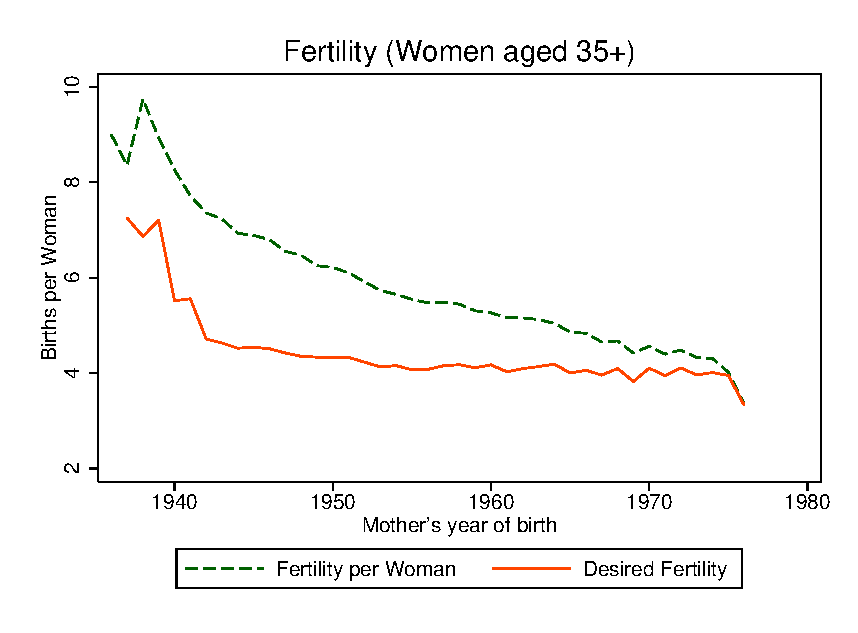
\includegraphics[scale=0.53]{\twinfolder/Figures/ferttrend_35_all.eps}
  \caption{Trends in Fertility}
  \label{TWINfig:fertrend}
\end{subfigure}%
\begin{subfigure}{.5\textwidth}
  \centering
  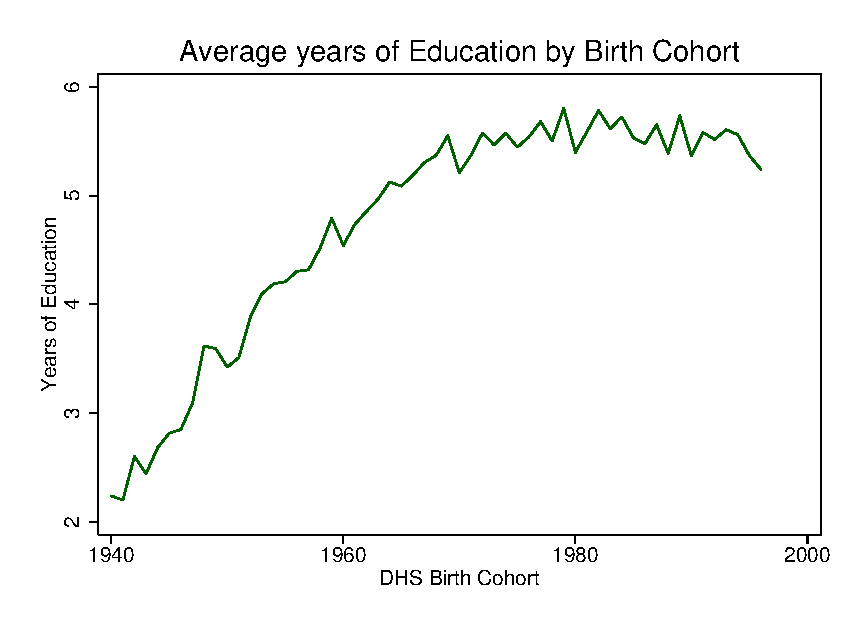
\includegraphics[scale=0.52]{\twinfolder/Figures/eductrend_all.eps}
  \caption{Trend in Education}
  \label{TWINfig:eductrend}
\end{subfigure}
\caption{Education and Fertility}
\label{TWINfig:trends}
\floatfoot{Note to figure \ref{TWINfig:trends}: Cohorts are made up of all individuals 
from the DHS who are over 35 years (for fertility), and over 15 years (for education).  
In each case the sample is restricted to those who have approximately completed fertility 
and education respectively.}
\end{figure}
\vspace{1cm}

\begin{figure}[htpb!]
\begin{center}
\caption{Proportion of Twins of All Births (USA)}
\label{TWINfig:bord}
\includegraphics[scale=0.92]{\twinfolder/Figures/USTwinFLE.eps} 
\end{center}
\end{figure}

\begin{figure}[htpb!]
\begin{center}
\caption{Twin Births and Total Fertility}
\label{TWINfig:births}
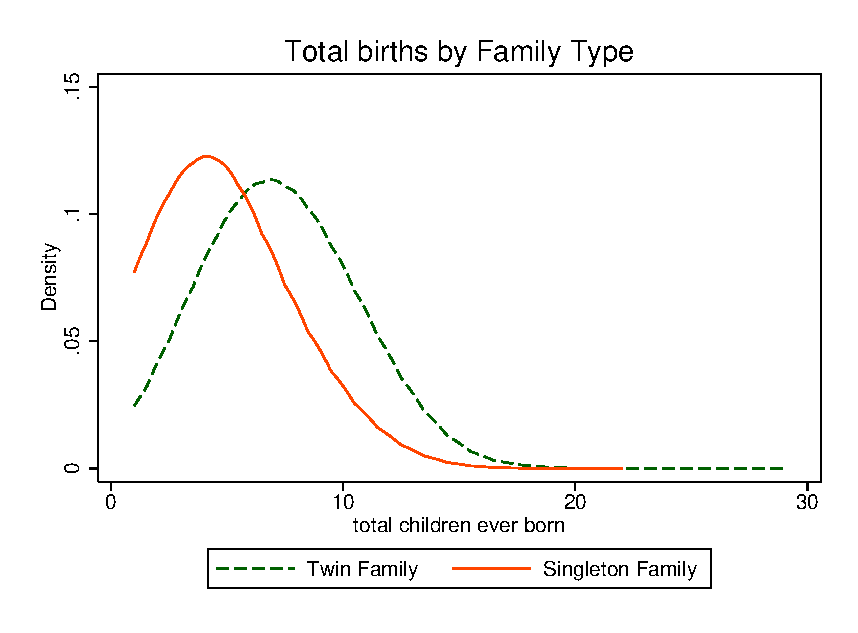
\includegraphics[scale=0.92]{\twinfolder/Figures/famsize.eps} 
\end{center}
\end{figure}

\begin{figure}[htpb!]
\begin{center}
\caption{Proportion of Twins by Birth Order}
\label{TWINfig:bord}
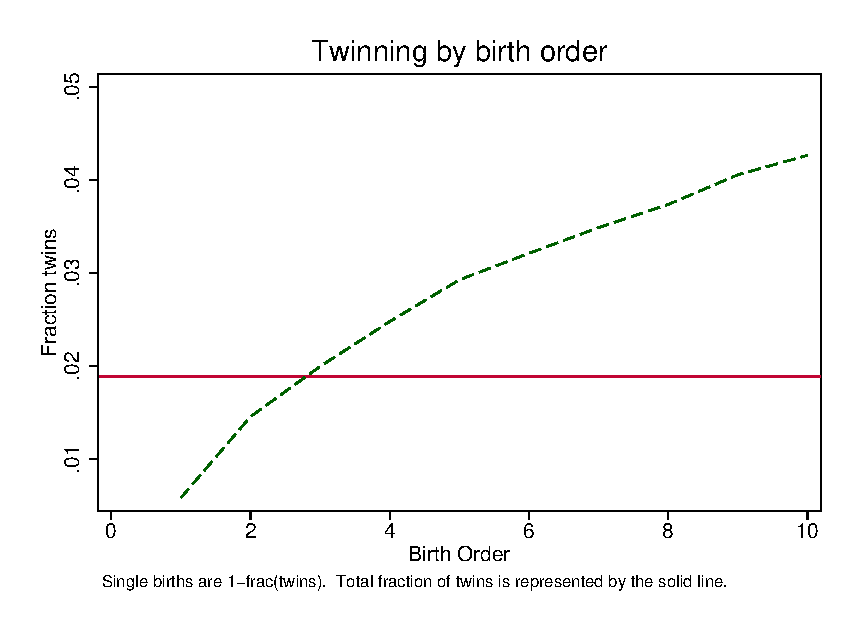
\includegraphics[scale=0.92]{\twinfolder/Figures/twinbybord.eps} 
\end{center}
\end{figure}

\begin{figure}[htpb!]
\begin{center}
\caption{Intra- and Inter-country trends: height and twinning}
\label{TWINfig:arrows}
\includegraphics[scale=0.86]{\twinfolder/Figures/height_country.eps} 
\end{center}
\end{figure}

%\begin{figure}[htpb!]
%\begin{center}
%\caption{Distribution of Ideal Family Size}
%\label{TWINfig:ideal}
%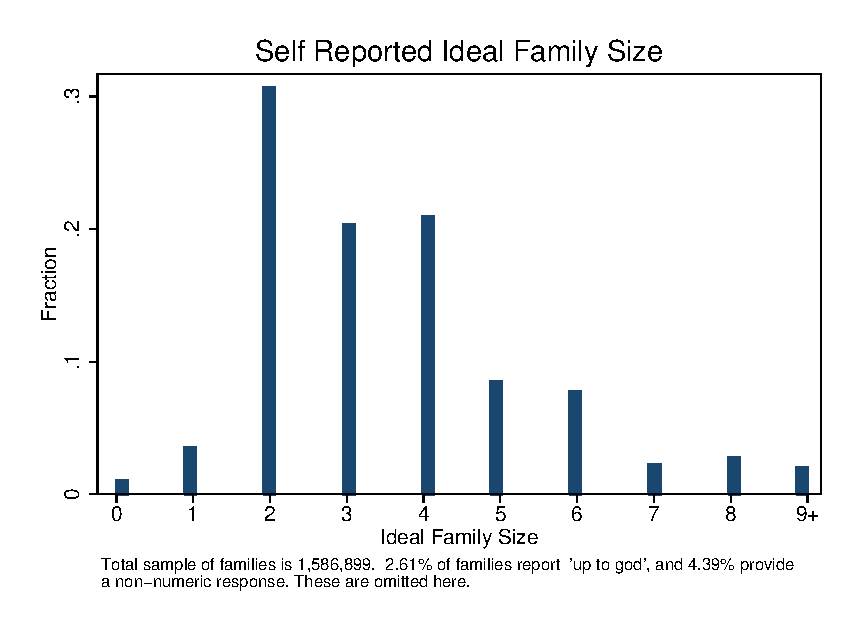
\includegraphics[scale=0.92]{\twinfolder/Figures/idealfamsize.eps} 
%\end{center}
%\end{figure}

%\begin{figure}[htpb!]
%\begin{center}
%\caption{Ideal and Actual Fertility}
%\label{TWINfig:idealactual}
%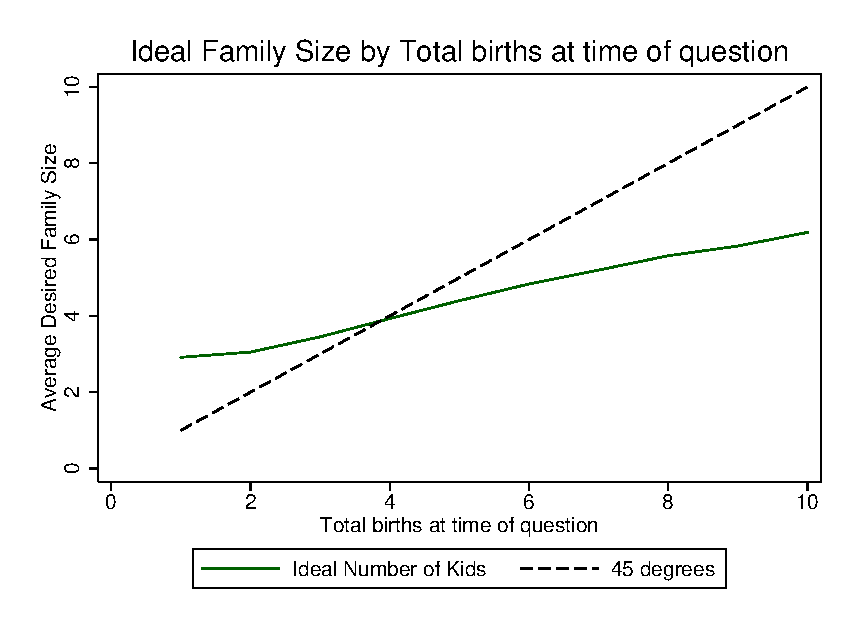
\includegraphics[scale=0.92]{\twinfolder/Figures/idealfam_fert.eps} 
%\end{center}
%\end{figure}

\begin{figure}[htpb!]
\begin{center}
\caption{Relaxing Strict Exogeneity (two plus)}
\label{TWINfig:ltz2}
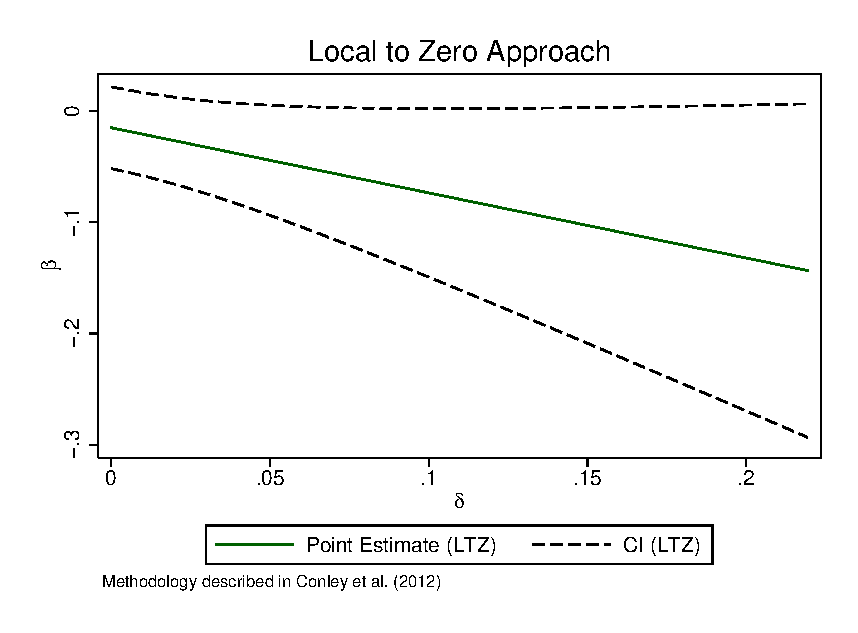
\includegraphics[scale=0.88]{\twinfolder/Figures/LTZ_two.eps}
\vspace{-8mm}
\floatfoot{Note to figure \ref{TWINfig:ltz2}: See note to Figure \ref{TWINfig:ltz3}}
\end{center}
\end{figure}

\begin{figure}[htpb!]
\begin{center}
\caption{Relaxing Strict Exogeneity (three plus)}
\label{TWINfig:ltz3}
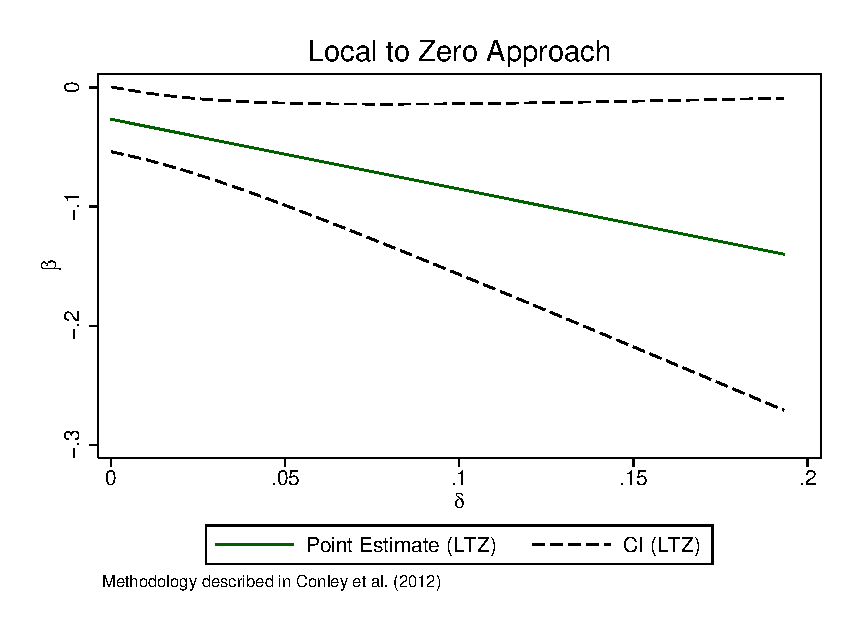
\includegraphics[scale=0.88]{\twinfolder/Figures/LTZ_three.eps} 
\floatfoot{Note to figure \ref{TWINfig:ltz3}: Confidence intervals and point estimates 
are calculated according to \citet{Conleyetal2012}.  Estimates reflect a range of priors 
regarding the validity of the exclusion restriction required to consistently estimate 
$\hat\beta_{fert}$ using twinning in a 2SLS framework.  The local to zero (LTZ) 
approach applied here assumes that $\gamma$, the sign on the instrument when included
in the first stage, is distributed $\gamma\sim U(0,\delta)$.  Further discussion 
is provided in the body of the text and table \ref{TWINtab:Conley}.}
\end{center}
\end{figure}




\clearpage
\section*{Tables}
\input{\twinfolder/Tables/BalanceBoth.tex}
\begin{landscape}\begin{table}[htpb!] 
\caption{Probability of Giving Birth to Twins} \label{TWINtab:twinreg1} 
\begin{center}\begin{tabular}{lcccccc} \toprule \toprule 
&(1)&(2)&(3)&(4)&(5)&(6)\\
Twin$\times$100&All&\multicolumn{2}{c}{Income}&\multicolumn{2}{c}{Time}&Prenatal\\
 \cmidrule(r){3-4} \cmidrule(r){5-6} 
&&Low inc&Middle inc&1990-2013&1972-1989&\\\midrule
\begin{footnotesize}\end{footnotesize}&\begin{footnotesize}\end{footnotesize}&\begin{footnotesize}\end{footnotesize}&\begin{footnotesize}\end{footnotesize}&\begin{footnotesize}\end{footnotesize}&\begin{footnotesize}\end{footnotesize}&\begin{footnotesize}\end{footnotesize}\\
Age&0.491***&0.489***&0.498***&0.587***&0.168***&0.632***\\
&(0.026)&(0.033)&(0.045)&(0.030)&(0.064)&(0.040)\\
Age Squared&-0.006***&-0.006***&-0.007***&-0.008***&-0.000&-0.009***\\
&(0.000)&(0.001)&(0.001)&(0.001)&(0.001)&(0.001)\\
Age First Birth&-0.051***&-0.082***&-0.002&-0.050***&-0.051***&-0.041***\\
&(0.008)&(0.010)&(0.013)&(0.009)&(0.015)&(0.013)\\
Education (years)&0.027*&0.065***&-0.008&0.044**&-0.008&-0.071**\\
&(0.016)&(0.021)&(0.027)&(0.019)&(0.028)&(0.028)\\
Education squared&-0.001&-0.005**&0.001&-0.002&0.002&0.003\\
&(0.001)&(0.002)&(0.002)&(0.001)&(0.002)&(0.002)\\
Height&0.057***&0.056***&0.058***&0.063***&0.038***&0.059***\\
&(0.004)&(0.005)&(0.006)&(0.005)&(0.007)&(0.007)\\
BMI&0.050***&0.059***&0.043***&0.046***&0.056***&0.045***\\
&(0.006)&(0.008)&(0.008)&(0.007)&(0.009)&(0.011)\\
Prenatal (Doctor)&&&&&&0.917***\\
&&&&&&(0.129)\\
Prenatal (Nurse)&&&&&&0.076\\
&&&&&&(0.109)\\
Prenatal (None)&&&&&&-0.479***\\
&&&&&&(0.133)\\
&&&&&&\\R-squared&0.01&0.01&0.01&0.01&0.00&0.01\\
Observations &2271948&1430703&841245&1660253&611695&624990\\
\hline\hline\multicolumn{7}{p{14.3cm}}{\begin{footnotesize}\textsc{Notes:} All specifications include a full set of year of birth and  country dummies, and are estimated as linear probability models.  Twin is multiplied by 100 for presentation.  Height is measured in cm  and BMI is weight in kg divided by height in metres squared. l  Prenatal care variables are only recoreded for recent births.  As  such, column (6) is estimated only for that subset of births where  these observations are made.
$^{*}$p$<$0.1; $^{**}$p$<$0.05; $^{***}$p$<$0.01
 \end{footnotesize}}\\ \hline \normalsize \end{tabular}\end{center}\end{table}\end{landscape} 

\begin{table}[htpb!]
\caption{Test of hypothesis that women who bear twins have better prior health}\label{TWINtab:IMR}\begin{center}\begin{tabular}{lccc}
\toprule \toprule 
\textsc{Infant Mortality (per 100 births)}& Base & +S\&H & Observations \\ \midrule 
\begin{footnotesize}\end{footnotesize}& 
\begin{footnotesize}\end{footnotesize}& 
\begin{footnotesize}\end{footnotesize}& 
\begin{footnotesize}\end{footnotesize}\\ 
Treated (2+)\hspace{5mm}\hspace{5mm}\hspace{5mm}\hspace{5mm}\hspace{5mm}\hspace{5mm}&-2.065***&-2.110***&503785\\
&(0.212)&(0.213)&\\
Treated (3+)\hspace{5mm}&-4.619***&-4.632***&686931\\
&(0.201)&(0.201)&\\
Treated (4+)&-4.257***&-4.243***&676303\\
&(0.183)&(0.183)&\\
Treated (5+)&-3.353***&-3.324***&587919\\
&(0.183)&(0.183)&\\
\midrule\multicolumn{4}{p{12.1cm}}{\begin{footnotesize}\textsc{Notes:} The sample for these regressions consist of all children who have been entirely exposed to the risk of infant mortality (ie those over 1 year of age). Subsamples 2+, 3+, 4+ and 5+ are generated to allow comparison of children born at similar birth orders.  For a full description of these groups see the the body of the paper or notes to table \ref{TWINtab:IVAll}. Treated=1 refers to children who are born before a twin while Treated=0 refers to children of similar birth orders not born before a twin.  Base and S+H controls are described in table \ref{TWINtab:IVAll}.$^{*}$p$<$0.1; $^{**}$p$<$0.05; $^{***}$p$<$0.01 
\end{footnotesize}} \\ \bottomrule 
\end{tabular}\end{center}\end{table}
\begin{table}[htpb]
\caption{Probability of Giving Births to Twins (NHIS, USA)}
\begin{center}
\scalebox{0.64}{
\begin{tabular}{lcc} \toprule
&(1)&(2) \\
VARIABLES&Twin$\times$100&Twin$\times$100 \\ \midrule
&& \\
Mother's Height&0.0416**&0.0406** \\
&(0.0201)&(0.0201) \\
Mother's Education&0.0084&0.0033 \\
&(0.0162)&(0.0164) \\
Smokes (pre-Pregnancy)&-0.119&-0.0983 \\
&(0.115)&(0.116) \\
Mother's Age&0.0121&0.0108 \\
&(0.0446)&(0.0446) \\
Mother's Age$^2$ &-0.0008&-0.0008 \\
&(0.0006)&(0.0006) \\
Age First Birth &0.166***&0.164*** \\
&(0.0135)&(0.0136) \\
BMI &0.0123***&0.0130*** \\
&(0.0034)&(0.0034) \\
Mother Good Health&&0.203* \\
&&(0.116) \\
Mother Poor Health&&-0.00284 \\
&&(0.189) \\
Constant&-4.091***&-4.101*** \\
&(1.542)&(1.543) \\
&& \\
Observations&105,879&105,879 \\
R-squared&0.004&0.004 \\ \midrule
%\multicolumn{3}{ p{5cm} }{\begin{footnotesize}\textsc{Notes:} Standard errors in parentheses. *** p$<$0.01; ** p$<$0.05; * p$<$0.1\end{footnotesize}}\bottomrule
\end{tabular}}
\end{center}
\end{table}



\input{\twinfolder/Tables/Alderman.tex}
\begin{landscape}
\input{\twinfolder/Tables/FDeath_Uncond.tex}
\end{landscape}
\input{\twinfolder/Tables/DHS-togetherAll.tex}
\begin{table}[htpb!]\caption{NHIS Estimates (USA): Education and Health}
\label{TWINtab:NHISAll}
\begin{center}
\scalebox{0.52}{
\begin{tabular}{lcccp{2mm}cccp{2mm}ccc}
\toprule \toprule 
&\multicolumn{3}{c}{2+}&&\multicolumn{3}{c}{3+}&&\multicolumn{3}{c}{4+}\\ \cmidrule(r){2-4} \cmidrule(r){6-8} \cmidrule(r){10-12} 
&Base&+H&+S\&H&&Base&+H&+S\&H&&Base&+H&+S\&H\\ \midrule 
\begin{footnotesize}\end{footnotesize}& 
\begin{footnotesize}\end{footnotesize}& 
\begin{footnotesize}\end{footnotesize}& 
\begin{footnotesize}\end{footnotesize}& 
\begin{footnotesize}\end{footnotesize}& 
\begin{footnotesize}\end{footnotesize}& 
\begin{footnotesize}\end{footnotesize}& 
\begin{footnotesize}\end{footnotesize}& 
\begin{footnotesize}\end{footnotesize}& 
\begin{footnotesize}\end{footnotesize}& 
\begin{footnotesize}\end{footnotesize}& 
\begin{footnotesize}\end{footnotesize}\\ 
\multicolumn{12}{l}{\textbf{OLS}}\\ 
School Z-Score&-0.043***&-0.033***&-0.027***&&-0.036***&-0.028***&-0.020**&&-0.010&-0.004&0.002\\
&(0.005)&(0.006)&(0.006)&&(0.008)&(0.009)&(0.009)&&(0.018)&(0.018)&(0.018)-\\
Excellent Health&-0.012***&-0.005***&-0.004*&&-0.018***&-0.010***&-0.008***&&-0.028***&-0.019***&-0.017***\\
&(0.002)&(0.002)&(0.002)&&(0.004)&(0.003)&(0.003)&&(0.006)&(0.005)&(0.005)\\

\begin{footnotesize}\end{footnotesize}&\begin{footnotesize}\end{footnotesize}&\begin{footnotesize}\end{footnotesize}&\begin{footnotesize}\end{footnotesize}&\begin{footnotesize}\end{footnotesize}&\begin{footnotesize}\end{footnotesize}&\begin{footnotesize}\end{footnotesize}&\begin{footnotesize}\end{footnotesize}&\begin{footnotesize}\end{footnotesize}&\begin{footnotesize}\end{footnotesize}&\begin{footnotesize}\end{footnotesize}&\begin{footnotesize}\end{footnotesize}\\
\multicolumn{12}{l}{\textbf{IV}}\\ 
School Z-Score&-0.064&-0.074&-0.077&&-0.027&-0.037&-0.036&&-0.094&-0.099&-0.113\\
&(0.063)&(0.059)&(0.058)&&(0.065)&(0.064)&(0.065)&&(0.152)&(0.155)&(0.150)\\

Excellent Health&0.013&0.022&0.019&&-0.016&-0.054*&-0.055*&&0.057&0.017&0.006\\
&(0.025)&(0.020)&(0.020)&&(0.038)&(0.031)&(0.031)&&(0.058)&(0.054)&(0.052)\\
\begin{footnotesize}\end{footnotesize}&\begin{footnotesize}\end{footnotesize}&\begin{footnotesize}\end{footnotesize}&\begin{footnotesize}\end{footnotesize}&\begin{footnotesize}\end{footnotesize}&\begin{footnotesize}\end{footnotesize}&\begin{footnotesize}\end{footnotesize}&\begin{footnotesize}\end{footnotesize}&\begin{footnotesize}\end{footnotesize}&\begin{footnotesize}\end{footnotesize}&\begin{footnotesize}\end{footnotesize}&\begin{footnotesize}\end{footnotesize}\\
\multicolumn{12}{l}{\textbf{Descriptives}}\\ 
School Z-Score&-0.0233&&&&-0.0363&&&&-0.0628&&\\
&(0.993)&&&&(1.041)&&&&(1.086)&&\\
Excellent Health&0.533&&&&0.511&&&&0.490&&\\
&(0.499)&&&&(0.500)&&&&(0.500)&&\\
\begin{footnotesize}\end{footnotesize}&\begin{footnotesize}\end{footnotesize}&\begin{footnotesize}\end{footnotesize}&\begin{footnotesize}\end{footnotesize}&\begin{footnotesize}\end{footnotesize}&\begin{footnotesize}\end{footnotesize}&\begin{footnotesize}\end{footnotesize}&\begin{footnotesize}\end{footnotesize}&\begin{footnotesize}\end{footnotesize}&\begin{footnotesize}\end{footnotesize}&\begin{footnotesize}\end{footnotesize}&\begin{footnotesize}\end{footnotesize}\\ 
Observations & 75,902 &	75,902 &	75,902 &&	57,413 &	57,413 &	57,413 &&	26,128 &	26,128 &	26,128 \\
Joint F-test Educ &&164.5&64.7&&&101.3&39.6&&&38.0&7.7\\
Joint F-test Health &&34469.6&163.9&&&15335.6&28.4&&&5276.4&17.1\\
\midrule\multicolumn{12}{p{20.6cm}}{\begin{footnotesize}\textsc{Notes:}  
Each cell presents the coefficient of interest from a regression using NHIS survey data (2002-2014). Base controls include child age FE (in months), mother's age, and mother's age at first birth 
plus race dummies for child and mother.  First stage omitted for clarity (generally all around 0.7).  Standard errors are clustered by mother.$^{*}$p$<$0.1; $^{**}$p$<$0.05; $^{***}$p$<$0.01. 
\end{footnotesize}} \\ \bottomrule 
\end{tabular}}\end{center}\end{table}

\input{\twinfolder/Tables/gamma.tex}
\begin{table}[htpb!]\caption{`Plausibly Exogenous' Bounds} 
\label{TWINtab:Conley}\begin{center}\begin{tabular}{lcccc}
\toprule \toprule 
&\multicolumn{2}{c}{UCI: $\gamma\in [0,\delta]$}&\multicolumn{2}{c}{LTZ: $\gamma \sim U(0,\delta)$}\\ 
\cmidrule(r){2-3} \cmidrule(r){4-5}
&Lower Bound&Upper Bound&Lower Bound&Upper Bound\\
Two Plus&-0.1860&0.0195&-0.1613&0.0011\\
Three Plus&-0.1710&0.0025&-0.1528&-0.0116\\
Four Plus&-0.1539&-0.0067&-0.1391&-0.0194\\
Five Plus&-0.1373&0.0277&-0.1215&0.0143\\
\midrule\multicolumn{5}{p{11.6cm}}{\begin{footnotesize}\textsc{Notes:} This table presents upper and lower bounds of a 95\% confidence interval for the effects of family size on (standardised) children's education attainment. These are estimated by the methodology of \citet{Conleyetal2012}  under various priors about the direct effect that being from a twin family has on educational outcomes ($\gamma$). In the UCI (union of confidence interval) approach, it is assumed the true $\gamma\in[0,\delta]$, while in the LTZ (local to zero) approach it is assumed that $\gamma\sim U(0,\delta)$.  In each case $\delta$ is estimated by including twinning in the first stage  equation and observing the effect size $\hat\gamma$.  Estimated $\hat\gamma$'s are (respectively for two plus to five plus):   0.1088, 0.0983, 0.0826, 0.0929.\end{footnotesize}}  
\\ \bottomrule \end{tabular}\end{center}\end{table} 

\clearpage


\bibliography{./BiBBase1}

\end{spacing}
\end{document}
